%%
%% This is file `sample-acmsmall.tex',
%% generated with the docstrip utility.
%%
%% The original source files were:
%%
%% samples.dtx  (with options: `acmsmall')
%% 
%% IMPORTANT NOTICE:
%% 
%% For the copyright see the source file.
%% 
%% Any modified versions of this file must be renamed
%% with new filenames distinct from sample-acmsmall.tex.
%% 
%% For distribution of the original source see the terms
%% for copying and modification in the file samples.dtx.
%% 
%% This generated file may be distributed as long as the
%% original source files, as listed above, are part of the
%% same distribution. (The sources need not necessarily be
%% in the same archive or directory.)
%%
%%
%% Commands for TeXCount
%TC:macro \cite [option:text,text]
%TC:macro \citep [option:text,text]
%TC:macro \citet [option:text,text]
%TC:envir table 0 1
%TC:envir table* 0 1
%TC:envir tabular [ignore] word
%TC:envir displaymath 0 word
%TC:envir math 0 word
%TC:envir comment 0 0
%%
%%
%% The first command in your LaTeX source must be the \documentclass
%% command.
%%
%% For submission and review of your manuscript please change the
%% command to \documentclass[manuscript, screen, review]{acmart}.
%%
%% When submitting camera ready or to TAPS, please change the command
%% to \documentclass[sigconf]{acmart} or whichever template is required
%% for your publication.
%%
%%
\documentclass[acmsmall,manuscript,screen,review,anonymous]{acmart}

%%
%% \BibTeX command to typeset BibTeX logo in the docs
\AtBeginDocument{%
  \providecommand\BibTeX{{%
    Bib\TeX}}}

%% Rights management information.  This information is sent to you
%% when you complete the rights form.  These commands have SAMPLE
%% values in them; it is your responsibility as an author to replace
%% the commands and values with those provided to you when you
%% complete the rights form.
\setcopyright{acmcopyright}
\copyrightyear{2018}
\acmYear{2018}
\acmDOI{XXXXXXX.XXXXXXX}


%%
%% These commands are for a JOURNAL article.
\acmJournal{JACM}
\acmVolume{37}
\acmNumber{4}
\acmArticle{111}
\acmMonth{8}

%%
%% Submission ID.
%% Use this when submitting an article to a sponsored event. You'll
%% receive a unique submission ID from the organizers
%% of the event, and this ID should be used as the parameter to this command.
%%\acmSubmissionID{123-A56-BU3}

%%
%% For managing citations, it is recommended to use bibliography
%% files in BibTeX format.
%%
%% You can then either use BibTeX with the ACM-Reference-Format style,
%% or BibLaTeX with the acmnumeric or acmauthoryear sytles, that include
%% support for advanced citation of software artefact from the
%% biblatex-software package, also separately available on CTAN.
%%
%% Look at the sample-*-biblatex.tex files for templates showcasing
%% the biblatex styles.
%%

%%
%% The majority of ACM publications use numbered citations and
%% references.  The command \citestyle{authoryear} switches to the
%% "author year" style.
%%
%% If you are preparing content for an event
%% sponsored by ACM SIGGRAPH, you must use the "author year" style of
%% citations and references.
%% Uncommenting
%% the next command will enable that style.
%%\citestyle{acmauthoryear}

% Comments
\newcommand{\mycomment}[2]{{\small\color{magenta}\underline{\sf{#1}}:} {\color{magenta}{\small #2}}}
\newcommand{\todo}[1]{\mycomment{Todo}{#1}}
\newcommand{\gcmt}[1]{\mycomment{Guan}{#1}}

% Shorthand
\newcommand{\Da}{\Downarrow}

% Unicode char
\usepackage{newunicodechar}
\newunicodechar{λ}{\lambda}
\newunicodechar{Σ}{\Sigma}
\newunicodechar{ρ}{\rho}
\newunicodechar{σ}{\sigma}
\newunicodechar{τ}{\tau}

% Semantics and reserved words
\mathchardef\mhyphen="2D
\usepackage[inference,ligature,reserved,shorthand]{semantic}
\reservestyle[\mathinner]{\command}{\mathit}
\command{let, in}
\command{true, false, bool, int, unit}
\command{pair, fst, snd, as}
\command{and, or, not, nand, nor, xor, for}
\command{if, then, else, while, print, fix, ref, var, when, do, end, robot, whereAmI, left, right, up, down}
\command{andf[and_f], andfp[and_f']}
\command{halfa[half\mhyphen adder], fulla[full\mhyphen adder], Rf[Ref]}

\reservestyle[\mathinner]{\Constructor}{\mathbf}
\Constructor{Bool, True, False}
\Constructor{Int, Lit, Plus, Eq, Lt}
\Constructor{Abs, App, Loc, Ref}

% Macro for Osazone semantics
\NewDocumentCommand{\branch}{ >{\SplitList{&}} m }{%
  \left(\begin{aligned} %
      \ProcessList{#1}{\brfunc}%
    \end{aligned}\right)%
}

\NewDocumentCommand{\brfunc}{m}{%
  & #1%
}

\newcommand{\lt}{\mathbf{let}}
\newcommand{\monad}{\mathbf{monad}~}
\newcommand{\as}{~\mathbf{as}~}

\newcommand{\Let}[2]{\lt~#1=#2;~}

\newcommand{\Exp}{\mathit{Exp}}
\newcommand{\Type}{\mathit{Type}}
\newcommand{\Id}{\mathit{Id}}
\newcommand{\Int}{\mathit{Int}}
\newcommand{\newLoc}{\mathit{newLoc}}
\newcommand{\store}{\mathit{store}}
\newcommand{\fetch}{\mathit{fetch}}
\newcommand{\return}{\mathit{return}}

\newcommand{\cqq}{\coloneqq}
\newcommand{\EE}[1]{\mathcal{E}(#1)}
\newcommand{\EEL}[1]{\mathcal{E}_{L}(#1)}
\newcommand{\EELL}[1]{\mathcal{E}_{L'}(#1)}
\newcommand{\TT}[1]{\mathcal{T}(#1)}
\newcommand{\TTL}[1]{\mathcal{T}_{L}(#1)}
\newcommand{\TTLL}[1]{\mathcal{T}_{L'}(#1)}

\mathlig{|>}{\triangleright}

\newcommand{\lifted}[1]{#1^\uparrow}
\newcommand{\ds}[1]{\mathbb{D}_1(#1)}
\newcommand{\DS}[1]{\mathbb{D}(#1)}
\newcommand{\DB}[1]{\mathbb{D}_b(#1)}
\newcommand{\dd}{\delta}
\newcommand{\dhl}[1]{\underline{\dd(#1)}}

\AtEndPreamble{%
\theoremstyle{acmdefinition}
\newtheorem{requirement}[theorem]{Requirement}
\newtheorem{assumption}[theorem]{Assumption}
}

\newcommand{\mE}{\mathcal{E}}
\newcommand{\mT}{\mathcal{T}}

\newcommand{\mexp}{\varepsilon}
\newcommand{\cexp}{\widetilde{\varepsilon}}
\newcommand{\ce}{\widetilde{e}}
\newcommand{\cb}{\widetilde{b}}

\newcommand{\STLC}{\textsc{Stlc}}
\newcommand{\STLCex}{\textsc{Stlc}$_\text{ex}$}
\newcommand{\RefIO}{\textsc{Ref}$_\text{IO}$}

\newcommand{\lr}{\rr{\phantom{E}}}  % ------>
\newcommand{\rr}[1]{\xrightarrow{~#1~}} % ---X-->

\newcommand{\miff}{\text{iff}}

\usepackage{tikz}
\usepackage{pifont}

%%
%% end of the preamble, start of the body of the document source.
\begin{document}

%%
%% The "title" command has an optional parameter,
%% allowing the author to define a "short title" to be used in page headers.
\title{Semantics Lifting for Domain-Specific Languages}

%%
%% The "author" command and its associated commands are used to define
%% the authors and their affiliations.
%% Of note is the shared affiliation of the first two authors, and the
%% "authornote" and "authornotemark" commands
%% used to denote shared contribution to the research.
\author{Zhichao Guan}
\email{guanzhichao@pku.edu.cn}
\author{Zhenjiang Hu}
\email{huzj@pku.edu.cn}
\affiliation{%
  \institution{School of Computer Science, Peking University}
  \city{Beijing}
  \country{China}
}
%%
%% By default, the full list of authors will be used in the page
%% headers. Often, this list is too long, and will overlap
%% other information printed in the page headers. This command allows
%% the author to define a more concise list
%% of authors' names for this purpose.
\renewcommand{\shortauthors}{Trovato et al.}

%%
%% The abstract is a short summary of the work to be presented in the
%% article.
\begin{abstract}
  A clear and well-documented \LaTeX\ document is presented as an
  article formatted for publication by ACM in a conference proceedings
  or journal publication. Based on the ``acmart'' document class, this
  article presents and explains many of the common variations, as well
  as many of the formatting elements an author may use in the
  preparation of the documentation of their work.
\end{abstract}

%%
%% The code below is generated by the tool at http://dl.acm.org/ccs.cfm.
%% Please copy and paste the code instead of the example below.
%%
\begin{CCSXML}
<ccs2012>
  <concept>
    <concept_id>10003752.10010124.10010131</concept_id>
    <concept_desc>Theory of computation~Program semantics</concept_desc>
    <concept_significance>500</concept_significance>
  </concept>
</ccs2012>
\end{CCSXML}
  
\ccsdesc[500]{Theory of computation~Program semantics}

%%
%% Keywords. The author(s) should pick words that accurately describe
%% the work being presented. Separate the keywords with commas.
\keywords{Programming Languages, Domain-Specific Languages}

\received{20 February 2007}
\received[revised]{12 March 2009}
\received[accepted]{5 June 2009}

%%
%% This command processes the author and affiliation and title
%% information and builds the first part of the formatted document.
\maketitle

\section{Introduction}

Language-oriented programming (LOP)\cite{LOP} is solving a class of problems by designing one or more new domain-specific languages (DSLs).
To avoid building common languages constructs like loops and branches,
developers may implement DSLs on top of another general-purpose programming language (called host language).
Developers can extend the host language based on the language features, rendering programs with domain-specific forms.
Languages with features like macros and higher-order functions are frequently employed.
By specifying translation rules from the DSL to the host language, developers can obtain a DSL interpreter naturally.
This type of DSL is called embedded DSL (eDSL).

Despite eDSL can significantly reduce implementation costs, DSL users find it inconvenient due to the inevitable need to learn the host language and understand error messages.
This is called abstraction leakage, where the users writes a program in DSL and it is translated into the host language,
causing the program executed formally differently from the original program.
Much prior work has focused on how to translate information from the host language to the DSL users manually.
\todo{More related work about generate information manually}

Pombrio et al. \cite{resugar} have made a great progress in maintenance of abstraction automatically.
They proposed \textit{resugaring}, by selectively reorganizing the sequence of evaluations on the host language to the DSL according to the reverse translation rules.
But there are several practical problems in this approach.
First, programs with a lot of syntactic sugars are pretty expensive to check whether each term in the evaluation sequences can be resugared.
Second, it still contains a host language evaluator executing,
so that users cannot intuit the functionality of language constructs.
Yang et al. \cite{lazy-desg} have solved the first problem via lazy desugaring.

% In this paper, we will focus on the second problem.
% In this paper, we propose a new approach to implementing DSLs by translation rules but make it standalone.

In general, embedded DSLs treat the host language as a black box.
We take the semantics of the host language as a white box, written by the meta language,
and derive the semantics for language constructs of DSL automatically.

We follow the core ideas of inferring type rules for syntactic sugars \cite{infer-types} and extend it to the semantics.
For example, in a host language with lambda abstraction and application, we can define $\<let>$ by translation rule:
\[ e_1~\<and>~e_2 => \<if>~e_1~\<then>~e_2~\<else>~\<false>. \]
The derivation of $\<and>$ is given in Fig. \ref{fig:and}.
In DSL, an expression matching the pattern of left-hand side (LHS) evaluates to $v$, if and only if the right-hand side (RHS) evaluates to $v$ (Step 1).
Based on the rules of if-then-else, we can futher expand the evaluation of RHS.
Since if-then-else is described in two rules according to the evaluation of $e_1$,
our derivation tree have to do the same thing (Step 2).
Similarly, the rule of $\<false>$ can be applied (Step 3).
Hence, we can obtain the following conclutions:
\[
  \inference{e_1 \Da \<true> & e_2 \Da v}
  {e_1~\<and>~e_2 \Da v}
  \qquad
  \inference{e_1 \Da \<false>}
  {e_1~\<and>~e_2 \Da \<false>}
\]
It should be observed that without mentioning $\<if>$, the rules directly describe the rules of $\<and>$.
That means, the abstraction we want to maintain --- that the rules of $\<and>$ are independent of the host language --- is true.

\begin{figure}[t!]
  \[
    \inference[(Step 1) ]{%
      \inference[(Step 2) ]{%
        e_1 \Da \<true>
        & e_2 \Da v
      }
      {\<if>~e_1~\<then>~e_2~\<else>~\<false> \Da v}
    }
    {e_1~\<and>~e_2 \Da v}
    \qquad
    \inference[(Step 1) ]{%
      \inference[(Step 2) ]{%
        e_1 \Da \<false>
        & \inference[(Step 3)]{}{\<false> \Da \<false>}
      }
      {\<if>~e_1~\<then>~e_2~\<else>~\<false> \Da \<false>}
    }
    {e_1~\<and>~e_2 \Da \<false>}
  \]
  \caption{Derivation of $\mathbf{and}$}
  \label{fig:and}
\end{figure}

It is seemingly natural but we are facing three challenges:
(1) Unlike type rules, which can typically be stated by one single rule,
many evaluation rules, such as $\<if>$, do not conform this property.
This may lead to nondeterminacy when searching rules or exponential growth in the number of rules.
(2) Most type rules are defined in a modular way,
which means the type of an expression depends on the types of subexpressions,
but the semantics may be not.
In particular, when using lambda-calculus as the host language,
lambda abstraction itself is a value.
Translation rules defined by lambda abstraction, is a value itself.
The evaluation rules of them may ruin the abstraction, like
\[ \<andf> => λx:\<bool>,y:\<bool>.~\<if>~x~\<then>~y~\<else>~\<false>. \]
(3) Since the rules of application include substitution,
we must specify the behavior of the expression containing substitution in semantic derivation.

To address challenge (1),
we introduce a variant of Skeleton \cite{skeleton} as meta-language to describe semantics.
Make sure that each language structure is evaluated according to unique rules,
in order to guarantee the determinacy of semantic derivation.
To address challenge (2),
we propose lambda lifting, to reveal the semantics of lambda abstraction.
To address challenge (3),
we show that substitution can maintain the correctness and abstraction of semantic derivation,
but we shall impose greater limitations on translation rules.

In this paper, we propose a new framework for DSL design.
We use simply-typed lambda-calculus (STLC) as the host language for its elementariness and versatility.
To increase the generality of the framework,
we provide meta-extensions (to introduce new vocabularies) and monad-extensions (to introduce side-effects) on the host language.
Then, users can specify DSL constructs by translation rules on the new extended host language.
Hence, as the focus of this paper, the framework will derive the evaluation rules and type rules for these constructs automatically, to make the DSL standalone.
All the semantics are described by the meta-language, and those of DSLs are generated.
Finally and naturally, our framework will generate interpreters based on semantics.
Our main technical contributions can be summarized as follows:

\begin{itemize}
  \item \todo{host}
  \item \todo{dsl}
  \item We present an algorithm to derive semantics for DSL constructs defined by translation rules.
        For the translation rules defined with lambda abstraction,
        we will give the lambda-lifting method.
        We will prove the correctness and abstraction of the algorithm.
  \item We give an implementation of the framework.
\end{itemize}

\section{Overview}

\begin{figure}
  \begin{tikzpicture}[x=6pt,y=6pt,yscale=1,xscale=1]

\draw[dashed] (-5,5) -- (23,5);
\node[align=left,fill=white] at (27,5) {Abstraction\\Barrier};

\node[draw] (H) at (0,0) {\STLC};
\node[draw] (D) at (0,10) {\textsc{Bool} };

\node[align=center,text=magenta] (M1) at (18,-1) {%
  $\EE{\mathit{if}~e_1~e_2~e_3} := \EE{e_1}: \left( \begin{aligned}
    & \mathit{true} \triangleright \EE{e_2} \\
    & \mathit{false} \triangleright \EE{e_3}
  \end{aligned}\right) $};

\node[align=center,text=magenta] (M2) at (18,11) {%
  $\EE{e_1~\mathit{and}~e_2} := \EE{e_1}: \left( \begin{aligned}
    & \mathit{true} \triangleright \EE{e_2} \\
    & \mathit{false} \triangleright \mathit{false}
  \end{aligned}\right) $};

\draw[->] (D) -> node[right=2pt,align=center,fill=white,pos=0.4] {$e_1~\<and>~e_2=>$\\$\<if>~e_1~e_2~\<false>$} (H);
\draw[->,thick,magenta] (18,1) -> node[left,fill=white,pos=0.6] {lifting} (18,9);
\draw[thick,magenta] (4,4) 
      to [out=-90,in=180] (6,2.5) 
      to (16,2.5) 
      to [out=0,in=-90] (18,4);

\end{tikzpicture}

  \caption{Semantics Lifting for \textsc{Bool}}
  \label{fig:bool-layer}
\end{figure}

% \begin{figure}[t!]
%   \begin{align*}
%     e \in \Exp  & ::= \<true> \mid \<false> \mid \<if>~e_1~e_2~e_3 \\
%                & \quad \mid x \mid λx:t.e \mid e_1~e_2            \\
%     t \in \Type & ::= \<bool> \mid t_1 -> t_2
%   \end{align*}
%   \caption{Syntax of \STLC}
%   \label{fig:stlc_syntax}
% \end{figure}

% \begin{figure}[t!]
%   \begin{align*}
%     e \in \Exp  & ::= \cdots \mid \<not>~e \mid e~\<and>~e \mid e~\<or>~e \\
%                 & \quad \mid e~\<nand>~e \mid e~\<nor>~e \mid e~\<xor>~e
%   \end{align*}
%   \caption{Syntax of \textsc{Bool}}
%   \label{fig:bool_syntax}
% \end{figure}

We start with a pretty simple example.
% to illustrate how we derive the semantics of the DSL defined by user through the translation rules.
Consider that developers would like to implement a DSL \textsc{Bool} to describe boolean operations.
Developers select \STLC{} as the host language.
We will show 
(1) how DSL developers define \textsc{Bool} by translation rules;
(2) how our algorithm lift the semantics of \textsc{Bool}.
Thereafter, if the developer wants to expand the language functionality
 and the host language is not expressive enough,
 the developer can extend the host language.

% So these operations can be defined using $\<if>$.
% For example, $\<and>$ operator can be defined by following translation rule:
% \[ e_1~\<and>~e_2 => \<if>~e_1~e_2~\<false> \]

% In this section, we will outline our approach with an example.
% And the following topics will be covered:
% (1) ;
% (2) how DSL becomes standalone by semantic lifting in our framework;
% and (3) how developers extend the host language by meta-extension.

% Consider that we take \STLC{} (whose syntax is shown in Fig. \ref{fig:stlc_syntax}) as the host language, 
%  and implement a DSL for boolean computations, named \textsc{Bool}.
% Programs in \textsc{Bool} are constructed by boolean values and operations, like:
% \begin{align*}
%   \<true>~\<and>~(\<false>~\<xor>~\<true>) & \equiv \<true> \\ 
%   (not~\<true>)~\<nor>~\<false> & \equiv \<true>.
%   % \<halfa>~\<true>~\<false> & \equiv (\<false>, \<true>).
% \end{align*}
% The syntax of \textsc{Bool} is shown in Fig. \ref{fig:bool_syntax},
%  where the syntax of \STLC{} is preserved.
%  and they are all treated as language constructs
%  for which we need to define there evaluation and type rules.

\subsection{Define \textsc{Bool} with Translation Rules}\label{sec:ov-1}

Boolean operations like $\<and>$ can be directly define by host language constructs like $\<if>$.
Each translation rule defines a new language construct in DSL.
And we require that each such language construct is determined by a unique translation rule.
A translation rule, ranged over by $tr$, consists of a LHS and a RHS splitted by $=>$,
 where LHS is an expression containing the new language construct and pattern variables;
 and RHS is composed of host language constructs and pattern variables.
Each pattern variable must be of a specific sort, such as $\Exp$, $\Type$.
We use $e_i$ for $\Exp$, $t_i$ for $\Type$, $x$ for identifiers.
Then, $\<and>$ can be defined as follows:
\[ e_1~\<and>~e_2 => \<if>~e_1~e_2~\<false> \]

\begin{figure}[t!]
  \begin{align*}
    \<not>~e        & => \<if>~e~\<false>~\<true> &
    e_1~\<or>~e_2   & => \<if>~e_1~\<true>~e_2 \\
    e_1~\<nand>~e_2 & => \<not>~(e_1~\<and>~e_2) &
    e_1~\<nor>~e_2  & => \<not>~(e_1~\<or>~e_2) \\
    \noalign{$e_1~\<xor>~e_2 => (e_1~\<and>~\<not>~e_2)~\<or>~(\<not>~e_1~\<and>~e_2)$}   
  \end{align*}
  \caption{Translation Rules for \textsc{Bool}}
  \label{fig:bool_tr1}
\end{figure}

Translation rules of the rest constructs in \textsc{Bool} are shown in Fig. \ref{fig:bool_tr1}.
In the example of $\<nand>$, DSL construct $\<not>$ and $\<and>$ is used in the translation rule.
This is permitted because we can think of these translation rules as being added to the host language one by one,
 i.e. $\<nand>$ is defined in a host language that contains $\<and>$ and $\<not>$.
But the translation rules defined recursively are illegal.

\subsection{Semantics Lifting for \textsc{Bool}}

Semantics lifting, or evaluation rules derivation,
 takes the rules of host language written by meta-language and a translation rule as input,
 and outputs the evaluation rules of the new language construct written by meta-language.
Therefore, before discussing the semantics lifting algorithm,
 we first briefly introduce the meta-language by example.
Consider the $\<if>$ construct with generic subexpressions denoted by $e_1$, $e_2$ and $e_3$,
 whose big-step operational semantics are defined using two seperate rules.
\[
  \inference{e_1 \Da \<true> & e_2 \Da v_2}
  {\<if>~e_1~e_2~e_3 \Da v_2} \quad
  \inference{e_1 \Da \<false> & e_3 \Da v_3}
  {\<if>~e_1~e_2~e_3 \Da v_3}
\]

In our meta-language, the evaluation of $\<if>$ expression is given by the following single rule:
\[
  \EE{\<if>~e_1~e_2~e_3} \cqq
  \EE{e_1}: \branch{
    \<true>  |> \EE{e_2} \\&
    \<false> |> \EE{e_3}
  }.
\]
Here, $\EE{e_1}$ identifies the evaluation of subexpression $e_1$,
 whose result is used to select a specific branch by pattern matching (after the colon).
Then, subsequent computations are processed (after the triangle).
If the value of $e_1$ is $\<true>$, then $e_2$ will be evaluate;
 the same for $\<false>$.
% All the evaluation rules can be expressed by recursive computations, meta-operations and branches.

Now it is time for our framework. 
Consider that for any $e_1$ and $e_2$,
 the value of $e_1~\<and>~e_2$ should be the same as $\<if>~e_1~e_2~\<false>$.
Hence, according to the translation rule and evaluation rules of the host language, we have
\begin{align*}
  \EE{e_1~\<and>~e_2} 
    & \cqq \EE{\<if>~e_1~e_2~\<false>} & \text{(Translation rule)} \\
    & = \EE{e_1}: \branch{
        \<true>  |> \EE{e_2} \\&
        \<false> |> \EE{\<false>}
      } & \text{(Evaluation rule of $\<if>$)} \\
    & = \EE{e_1}: \branch{
        \<true>  |> \EE{e_2} \\&
        \<false> |> \<false>
      } & \text{(Evaluation rule of $\<false>$)} 
\end{align*}
The evaluation rule of $\<and>$ has been derived.
The following points are worth noting:
(1) Abstraction: the semantics of $\<and>$ is made explicit, and no longer needs to be expressed by $\<if>$ from the host language.
That is, even if we remove $\<if>$ from the language, the $\<and>$ works fine. (Fig. \ref{fig:bool-layer})
(2) Uniqueness: due to our requirement of uniqueness of the rules, 
 the rule unfolding in the derivation is always deterministic.
Also thanks to uniqueness of translation rules,
 the rules we derive for these new language constructs stay unique.

The typing rule can also be derived in a similar way, and we will not discuss this in detail.
%  and we will not elaborate on them here.

\paragraph{Lambda Lifting.}
As mentioned above, a language construct can be defined as a lambda abstraction by translation rules, like $\<andf>$.
The above method will result in a rule which which breaks abstraction:
\begin{align*}
  \EE{\<andf>} 
    & \cqq \EE{λx:\<bool>.~λy:\<bool>.~\<if>~x~y~\<false>} \\
    & = λx:\<bool>.~λy:\<bool>.~\<if>~x~y~\<false>, 
\end{align*}
But by converting $\<andf>$ to $\<and>$, the internal computation can be exposed.
The approach of exposing parameters of the lambda abstraction in RHS,
 and transforming the rule into a set of new translation rules, is called lambda lifting.
In the above example, $\<andf>$ will be transformed into the following two rules:
\begin{align*}
  \mathit{and_f'}~e_1~e_2 & => \<if>~e_1~e_2~\<false> \\ 
  \<andf> & => λx:\<bool>.~λy:\<bool>.~\mathit{and_f'}~x~y.
\end{align*}
By thinking of $\mathit{andf'}$ as a language construct on the DSL,
 the abstraction property of $\<andf>$ is satisfied.
Lambda lifting plays an import role in translation rules with nested lambda abstractions.

% \paragraph{Derive the type rules.}
% The method of deriving evaluation rules can also be applied to type rules.
% For example, the type rule of $\<and>$ can be derived by
% \begin{align*}
%   \TT{e_1~\<and>~e_2}
%     & \cqq \TT{\<if>~e_1~e_2~\<false>} 
%         & \text{(Translation rule)} \\
%     & = \Let{\<bool>}{\TT{e_1}}
%         \Let{t_2}{\TT{e_2}}
%         \TT{\<false>}:(t_3 \mid t_2 = t_3 |> t_2)
%         & \text{(Evaluation rule of $\<if>$)} \\
%     & = \Let{\<bool>}{\TT{e_1}}
%         \Let{t_2}{\TT{e_2}}
%         \<bool>:(t_3 \mid t_2 = t_3 |> t_2)
%         & \text{(Evaluation rule of $\<false>$)} \\
%     & = \Let{\<bool>}{\TT{e_1}}
%         \Let{\<bool>}{\TT{e_2}}
%         \<bool>.
%         & \text{(Simplification)}
% \end{align*}



% \subsection{Define Host Language via Meta-Language}

% Skeletal semantics \cite{skeleton} can be used to describe concrete and abstract semantics in a structural way.
% A skeleton body is defined by a sequence of bones.
% A bone is either recursive computations (hooks),
%  meta-operations (filters), or different pathways (branches).
% Our meta-language is based on Skeleton, but for different goals.
% We replace branch and merging with pattern matching,
%  and replace filters with meta-functions.
% For example, consider the $\<if>$ construct with generic subexpressions denoted by $e_1$, $e_2$ and $e_3$,
%  whose big-step operational semantics are defined using two seperate rules.
% \[
%   \inference{e_1 \Da \<true> & e_2 \Da v_2}
%   {\<if>~e_1~e_2~e_3 \Da v_2} \quad
%   \inference{e_1 \Da \<false> & e_3 \Da v_3}
%   {\<if>~e_1~e_2~e_3 \Da v_3}
% \]
% In our meta-language, the evaluation rule of $\<if>$ is given by
% \[
%   \EE{\<if>~e_1~e_2~e_3} \cqq
%   \EE{e_1}: \branch{
%     \<true>  |> \EE{e_2} \\&
%     \<false> |> \EE{e_3}
%   }.
% \]
% Here, $\EE{e_1}$ identifies the evaluation of subexpression $e_1$,
%  whose result is used to select a specific branch by pattern matching (after the colon).
% Then, subsequent computations are processed (after the triangle).
% If the value of $e_1$ is $\<true>$, then $e_2$ will be evaluate; the same for $\<false>$.
% The typing rule of $\<if>$ can be defined in a similar way:
% \[
%   \TT{\<if>~e_1~e_2~e_3} \cqq
%     \lt~\<bool> = \TT{e_1};~
%     \lt~t_2 = \TT{e_2};~
%   \TT{e_3}:(t_3 \mid t_2 = t_3 |> t_2)
% \]
% In order to make the structure clear,
% we use $let$ as a syntactic sugar to represent a pattern matching with unique branch.
% The type of $e_1$ is required to be $\<bool>$.
% The matching of $e_3$ has a side condition (named \textit{guard} in Haskell),
% which requires $t_2$ to equal $t_3$.
% Note that the evaluation and typing rules of $\<if>$ are unique,
%  which guarantees the determinacy in derivation.
 


% \begin{figure}[t!]
%   \begin{align*}
%     \EE{\<true>}           & \cqq \<true>                                              \\
%     \EE{\<false>}          & \cqq \<false>                                             \\
%     \EE{\<if>~e_1~e_2~e_3} & \cqq \EE{e_1}: \branch{
%       \<true>  |> \EE{e_2}                                                               \\&
%       \<false> |> \EE{e_3}
%     }                                                                                  \\
%     \EE{λx:t.e}            & \cqq λx:t.e                                               \\
%     \EE{e_1~e_2}           & \cqq \lt~λx:t.e=\EE{e_1};~\lt~v_2=\EE{e_2};~\EE{e[v_2/x]}
%   \end{align*}
%   \caption{Semantics of \STLC}
%   \label{fig:stlc}
% \end{figure}

% The syntax of \STLC{} is given in Fig. \ref{fig:stlc_syntax}.
% And the semantics of \STLC{} is given in Fig. \ref{fig:stlc}.
% But meta-language focus on the semantics rather than syntax.
% We need to think of each item of syntax as a language construct.
% In the evaluation rules, we can observe that:
% (1) the evaluation of values gets themselves,
%  which is consistent with the big-step operational semantics,
% (2) and we use substitution in application.
% In our meta-language, substitution is considered as a special meta-function.
% The substitution rules of language constructs should be specified by developers, omitted here.

% We can think of evaluation $\mathcal{E}$ as a function of $\Exp -> \Exp$.
% Then the type $\mathcal{T}$ should be a function of $\Exp -> \Type$.
% But a context is necessary when typing lambda abstraction.
% Instead of changing $\mathcal{T}$ to $\Exp -> Ctx -> \Type$,
% we introduce state monad to describe context modification for modularity.
% So that $\mathcal{T}$ is a function of $\Exp -> State~CtxStack~\Type$.
% \todo{How to explain this monad more clearly?}
% \[
%   \TT{λx:t.e} \cqq \lt~\_=updateCtx~x~t;~\lt~t'=\TT{e};~\lt~\_=restoreCtx;~t->t'
% \]

% With the Introduction of monad, the type rule of $\<if>$ remains unchanged.
% We can also keep the original semantic description intact
% when subsequent DSL users extend the host language.
% The type rules of \STLC is given in Fig. \ref{fig:stlc_type}.

% \begin{figure}[t!]
%   \begin{align*}
%     \TT{\<true>}  & \cqq \<bool>  \\
%     \TT{\<false>} & \cqq \<bool>  \\
%     \TT{\<if>~e_1~e_2~e_3} & \cqq
%       \lt~\<bool> = \TT{e_1};~
%       \lt~t_2 = \TT{e_2};~
%       \TT{e_3}:(t_3 \mid t_2 = t_3 |> t_2)   \\
%     \TT{x}        & \cqq searchCtx~x \\
%     \TT{λx:t.e}   & \cqq \lt~\_=updateCtx~x~t;~\lt~t'=\TT{e}; \\
%                   & \hspace{13pt} \lt~\_=restoreCtx;~t->t' \\
%     \TT{e_1~e_2}  & \cqq \Let{t_1->t}{\TT{e_1}} \TT{e_2}:(t_2\mid t_1=t_2|>t)
%   \end{align*}
%   \caption{Type Rules of \STLC}
%   \label{fig:stlc_type}
% \end{figure}

\subsection{Extend the host language}

Consider that developers would like to support $\<halfa>$ and $\<fulla>$ in the \textsc{Bool} language.
For example:
\[ \<halfa>~\<true>~\<false> \equiv (\<false>, \<true>) \]
However, they cannot be implemented by translation rules,
 because half adder and full adder will get a pair of sum and carry as the results. 
Pairs are in demand to build compound data structures.
Naturally, projection $\<fst>$ and $\<snd>$ are involved as $\Exp$,
 and product $t \times t$ is involved as $\Type$.
Developers need to indicate the evaluation and typing rules for each newly defined language constructs, as shown in Fig. \ref{fig:bool-meta-ex}.

\begin{figure}[t!]
  \begin{align*}
    \EE{(e_1,e_2)} & \cqq \lt~v_1=\EE{e_1};~\lt~v_2=\EE{e_2};~(v_1,v_2) &
    \TT{(e_1,e_2)} & \cqq \lt~t_1=\TT{e_1};~\lt~t_2=\TT{e_2};~t_1\times t_2 \\
    \EE{\<fst>~e} & \cqq \lt~(v_1,\_)=\EE{e};~v_1 &
    \TT{\<fst>~e} & \cqq \lt~(t_1,\_)=\TT{e};~t_1 \\
    \EE{\<snd>~e} & \cqq \lt~(\_,v_2)=\EE{e};~v_2 &
    \TT{\<snd>~e} & \cqq \lt~(\_,t_2)=\TT{e};~t_2
  \end{align*}
  \caption{Meta-Extension Rules for \textsc{Bool}}
  \label{fig:bool-meta-ex}
\end{figure}

Based on this host language with meta-extension,
 $\<halfa>$ and $\<fulla>$ can be defined by translation rules.
The new translation rules are shown in Fig. \ref{fig:bool_adder}.
And the evaluation rules of these language constructs can be derived using the above algorithm.

\begin{figure}[t!]
  % \begin{align*}
  %   e \in \Exp  & ::= \cdots \mid (e,e) \mid \<fst>~e \mid \<snd>~e \\
  %               & \quad \mid \<halfa>~e~e \mid \<fulla>~e~e~e \\
  %   t \in \Type & ::= \cdots \mid t\times t
  % \end{align*}
  \begin{align*}
    \<halfa>~e_1~e_2 & => (e_1~\<xor>~e_2,e_1~\<and>~e_2) \\
    \<fulla>~e_1~e_2~e_3 & => (e_1~\<xor>~e_2~\<xor>~e_3, (e_1~\<xor>~e_2)~\<or>~(e_3~\<and>~(e_1~\<xor>~e_2)))
  \end{align*}
  \caption{Syntax of \textsc{Bool} with Adders and New Translation Rules}
  \label{fig:bool_adder}
\end{figure}

\section{Meta-Language and Host Languages}\label{sec:host}

In this section, we formalize the syntax and semantics of our meta-language (Section \ref{sec:meta}).
The meta-language is used to define the semantics and typing rules of languages.
We define \STLC{} with this meta-language as an instance.
Then we want to emphasize the importance of structural evaluation rules of host language,
 in preparation for the semantics derivation (Section \ref{sec:m-host}).
Note the difference between concepts of meta-language and host languages (or any language defined by meta-language) in this section.
We use $L$ to refer to a language defined by meta-language like \STLC.
In the remainder of this section, we will indicate such language with an $L$ to distinguish from the meta-language.

\subsection{Meta-Language}\label{sec:meta}

Our meta-language is inspired by Skeleton \cite{skeleton}, 
 used to describe concrete and abstract semantics in a structural way.
A skeleton body is defined by a sequence of bones.
A bone is either recursive computations (hooks), filters, or branches.
Skeleton focuses on illustrating the consistency of concrete and abstract interpretations.
The meaning of filters varies in different goals.
But our meta-language concentrate on evaluation and typing,
 whose design is intuitively close to Haskell.
In particular, we replace branches and merging operation with pattern matching,
 and replace filters with meta-functions.
In addition, monad is supported to cover side effects in meta-language. % at the meta-language level.

\todo{Overview of this subsection: language, rule, expression}
\[   \EE{e_1~\<and>~e_2} \cqq \EE{e_1}: \branch{
    \<true>  |> \EE{e_2} \\&
    \<false> |> \<false> } \]

\subsubsection{Expressions of Meta-Language}
Various \textit{expressions} in the meta-language are used to encode the language constructs in the host language or the DSL, such as expressions and types.

An expression $\mexp$ is built by \textit{base expressions}, like literals and identifiers, ranged over by $\mexp_b$;
 \textit{expression variables}, ranged over by $\mexp_x$;
 and \textit{compound expressions} by \textit{constructors}, ranged over by $c$.
Each language construct in $L$ corresponds to a constructor $c$ in meta-language.
To distinguish between various sorts of language constructs,
 we define $S$ for a finite set of \textit{sorts}, ranged over by $s$.
A sort $s$ can be either an \textit{base sort} like $\Int$, $\Id$;
 or a \textit{program sort} like $\Exp$, $\Type$ in \STLC.
The sort of an expression $\mexp$, written as $sort(\mexp)=s$,
 illustrates its role in language $L$.
A constructor $c$ has a signature $sig(c)$, which is of the form $(s_1\cdots s_n)->s$,
 where $s_1\cdots s_n$ are appropriate sorts of parameters of $c$,
 and $s$ is the sort of expressions constructed by $c$, briefly stated as sort of $c$.
A compound expression, written as $c(\mexp_1,\cdots,\mexp_n)$ or $c~\mexp_1\cdots\mexp_n$,
 is valid, if $sort(\mexp_i)=s_i$ for each $i\in [1..n]$.

\begin{example}
Expression $λx\!\!:\!\!\<bool>.~e$ in language $L$, is constructor $\<Abs>$ applied to ``x'', $\<bool>$ and expression variable $e$.
 ``x'' is a base expression, and $sort(``x")=\Id$;
 $\<bool>$ is constructor $\<Bool>$ applied to nothing.
The signature of $\<Abs>$ is $sig(\<Abs>)=(\Id,\Type,\Exp)->\Exp$, and its sort is $\Exp$.
The signature of $\<Bool>$ is $()->\Type$, and its sort is $\Type$.
\[
  \begin{array}{ccc}
    % \text{Language } L & & \text{Meta-Language} \\
    λx\!:\<bool>.~e & \leftrightarrow & \<Abs>(``x",\<Bool>(),e) \text{ or } \<Abs>~``x"~\<Bool>~e
  \end{array}
\]
\end{example}

We use $i$ for expressions with sort $\Int$, $x$ for $\Id$, $e$ for $\Exp$, and $t$ for $\Type$.
A \textit{closed expression} $\cexp$ is an expression with no expression variables, generally refering to a concrete component in language $L$.
Let $Σ$ be an \textit{environment} mapping from expression variables to expressions. 
We write $Σ(\mexp)$ to replace all expression variables $\mexp_x\in dom(Σ)$ with $Σ(\mexp_x)$ in $\mexp$.
An environment $Σ$ is \textit{closed} for expression $\mexp$, when $Σ(\mexp)$ is a closed expression.

\subsubsection{Rules of Meta-Language}

\begin{figure}
  \begin{align*}
    b \in Bone 
      & ::= \mexp' & \text{(Pure Expression)} \\
      & \quad \mid h(\mexp') & \text{(Recursive Computation)} \\
      & \quad \mid f_m(\mexp'_1\cdots \mexp'_n) & \text{(Monadic Meta-function)} \\
      & \quad \mid b:(br_1\cdots br_n) & \text{(Pattern Matching)} \\
      & \quad \mid \Let{pat}{b_1} b_2 & \text{(Let Binding)} \\
    \mexp' \in \Exp_P
      & ::= \mexp & \text{(Expression)} \\
      & \quad \mid f_p(\mexp'_1\cdots \mexp'_n) & \text{(Pure Meta-function)} \\
    br \in Branch
      & ::= pat |> b \\
      & \quad \mid pat \mid \mexp' |> b \\
    pat \in \mathit{Pattern}
      & ::= \mexp_x & \text{(Pattern Variable)} \\
      & \quad \mid c~pat_1\cdots pat_n & \text{(Compound Pattern)}
  \end{align*}
\caption{Body of Rules in Meta-Language}
\label{fig:body}
\end{figure}

A rule of meta-language has the shape $h(c~\mexp_{x_1}\cdots \mexp_{x_n}) \cqq b$, 
 where $h$ is the name of interpretation like $\mathcal{E}$ and $\mathcal{T}$,
 $c$ is a constructor, 
 $\mexp_{x_1}\cdots \mexp_{x_n}$ are expression variables,
 and $b$ is the rule body.
An interpretation $h$ has a signature of the form $s_1->m~s_2$, 
 written as $sig(h)=s_1->m~s_2$ or $h:s_1->m~s_2$, 
 where $s_1$ states for which $h$ computes,
 and $s_2$ states for the result of $h$,
 $m$ is the monad for side-effects.
When no side effects are introduced, $m$ can be omitted.
The rule body is composed of bones, shown in Fig. \ref{fig:body}.
A bone, which represents a step of operation, 
 can be either a pure expression,
 a recursive computation,
 or a meta-function.

\begin{example}
  The typing rule of $\<if>$ is defined as follows:
  \[
    \TT{\<if>~e_1~e_2~e_3} \cqq
      \lt~\<bool> = \TT{e_1};~
      \lt~t_2 = \TT{e_2};~
    \TT{e_3}:(t_3 \mid t_2 = t_3 |> t_2)
  \]
  We use $let$ as a syntactic sugar to represent a pattern matching with only one branch.
  In this rule, the type of $e_1$ is required to be $\<bool>$.
  The matching of $\TT{e_3}$ has a side condition (named \textit{guard} in Haskell),
  which requires $t_2=t_3$.
\end{example}

Pure expressions are expressions $\mexp$ or computation results of pure meta-function $f_p$.
The meta-functions represent primitive operations, and we assume that users can always understand their meaning, like equality checking $(=)$.
Most of these functions are pre-defined.
Two types of meta-functions are mentioned here:
 monadic meta-functions, ranged over by $f_m$,
 pure meta-functions, ranged over by $f_p$.
They are the same if the interpretation is pure.
When monad is introduced,
 $f_m$ is function containing side effects, 
  whose signature is like $sig(f_m)=(s_1\cdots s_n)->m~s$;
 while $f_p$ is not,
  whose signature is like $sig(f_p)=(s_1\cdots s_n)->s$.
% For example, $searchCtx$, $updateCtx$ and $restoreCtx$ are monadic meta-functions,
%  equality checking $(=)$ and substitution are pure meta-functions.

A \textit{closed bone} $\cb$ is a bone without any free expression variables,
 which can be reduced to an expression.
Also, we extend the environment to bone as $Σ(b)$, which replaces free expression variables in $dom(Σ)$.

In our meta-language, $\mathit{return}$ or $\mathit{bind}$ in the body of rules are used implicit.
An expression variable bound with sort $m~s$ is not allowed.
As a result, the method to tell whether a binding is pure is by checking if the bone is a pure expression.
\todo{not clear?}

\subsubsection{Language $L$ Defined in Meta-Language}
A \textit{Language} $L$ consists of a set of program sorts $S_p$;
 a set of language constructs $C$ with signatures;
 a set of interpretations $H$ with rules;
 a set of meta-functions $F$, devided into monadic ones $F_m$ and pure ones $F_p$.

In particular, in \STLC{}, $S_p=\{\Exp,\Type\}$.
$H$ can be seperated into a set of evaluation rules $R_{\mE}$ and a set of typing rules $R_{\mT}$.
The evaluation rules of \STLC{} are defined in Fig. \ref{fig:stlc} where $\mE:\Exp->\Exp$.
But when typing \STLC, a context (or environment) mapping variables to types is necessary.
Instead of making the signature $\mT$ be $\Exp -> Ctx -> \Type$,
 we introduce state monad to describe context modification\footnote{
  A more direct approach is to use the reader monad and change the environment locally via $\mathit{local}$.
  But $\mathit{local}$ needs a monadic computation as argument, which is not allowed.
 },
 with monadic meta-functions $searchCtx$, $updateCtx$ and $restoreCtx$.
When typing lambda abstractions $λx:t.e$, the type of variable $x$ should be updated into context first with $updateCtx$.
After typing the body of lambda abstractions $e$, restore the type of variable $x$ in the context.
In the concrete implementation, the stack of the context is used as the state.
When searching for the type of a variable, the context at the topmost level is looked up.
Updating the context will push the new context onto the stack and restoring will pop one.
So the signature of $\mT$ is modified to $\Exp -> (State~\mathit{CtxStack})~\Type$.
And the typing rules are defined in Fig. \ref{fig:stlc_type}.

\begin{figure}[t!]
  \begin{align*}
    \EE{\<true>}           & \cqq \<true> \\
    \EE{\<false>}          & \cqq \<false> \\
    \EE{\<if>~e_1~e_2~e_3} & \cqq \EE{e_1}: \branch{
      \<true>  |> \EE{e_2} \\&
      \<false> |> \EE{e_3}
    } \\
    \EE{λx:t.e}            & \cqq λx:t.e \\
    \EE{e_1~e_2}           & \cqq \lt~λx:t.e=\EE{e_1};~\lt~v_2=\EE{e_2};~\EE{e[v_2/x]}
  \end{align*}
  \caption{Evaluation Rules of \STLC}
  \label{fig:stlc}
\end{figure}

\begin{figure}[t!]
  \begin{align*}
    \TT{\<true>}  & \cqq \<bool>  \\
    \TT{\<false>} & \cqq \<bool>  \\
    \TT{\<if>~e_1~e_2~e_3} & \cqq
      \lt~\<bool> = \TT{e_1};~
      \lt~t_2 = \TT{e_2};~
      \TT{e_3}:(t_3 \mid t_2 = t_3 |> t_2)   \\
    \TT{x}        & \cqq searchCtx~x \\
    \TT{λx:t.e}   & \cqq \lt~\_=updateCtx~x~t;~\lt~t'=\TT{e}; \\
                  & \hspace{13pt} \lt~\_=restoreCtx;~t->t' \\
    \TT{e_1~e_2}  & \cqq \Let{t_1->t}{\TT{e_1}} \TT{e_2}:(t_2\mid t_1=t_2|>t)
  \end{align*}
  \caption{Typing Rules of \STLC}
  \label{fig:stlc_type}
\end{figure}

Substitution, as a pure meta-function, is divided from $F_p$ and described as a set of substitution rules $R_{subst}$.
The signature of substitute is $sig(subst)=(\Exp,\Id,\Exp)->\Exp$.
The substitution rules of language constructs should be specified by developers, omitted here.

In the rest of this paper, a language (\STLC{} or its extensions) are presented as follows:
\[ L=\langle S_p, C, R_{\mE}, R_{\mT}, R_{subst}, F_p, F_m \rangle \]

\begin{requirement}
  For any constructor $c$ with sort $\Exp$, the evaluation rule, the typing rule and the substitution rule in $L$ should be unique.
  % (Variable has no evaluation rules.)
\end{requirement}

When a closed expression $\cexp$ is evaluated (or typed) in $L$,
 we need to find a rule in $L$ and apply it to $\cexp$.
We write $L[\cexp]_{\mE}=Σ(b)$, if there exists a rule $\mE(c~\mexp_{x_1}\cdots \mexp_{x_n}) \cqq b$ in $R_{\mE}$ and an environment $Σ$,
 so that $\cexp=Σ(c~\mexp_{x_1}\cdots \mexp_{x_n})$.

% L[e]

\subsubsection{Semantics of Meta-Language}

In this section, we present the semantics of our meta-language.
We start by the pure computation.
Given a closed expression $\cexp$ in language $L$, for an interpretation $h$,
 whose sort is $s_1 -> s_2$, if $sort(\cexp)=s_1$, 
 then $h(\cexp)$ will be computed to get a closed expression of sort $s_2$.
% For example, an expression is interpreted as a value if $h$ is evaluation, written as $\cexp -> v$.
% Here we use $v$ for the result of interpretation, which is a closed expression itself.
After monad is introduced, side effects can be embraced by labels in transformation \cite{msos}.
The operational semantics of meta-language are given in Fig. \ref{fig:seman-meta}.
\todo{Explain this in detail?}

\begin{figure}
  \begin{gather*}
    \inference[Base]{}{\mexp_b \lr \mexp_b} \\
    \inference[PureFun]{\mexp'_1 \lr v_1 ~\cdots~ \mexp'_n \lr v_n & v=f_p(v_1\cdots v_n)}{f_p(\mexp'_1\cdots \mexp'_n) \lr v} \\
    \inference[Rec]{\mexp' \lr v_1 & L[v_1]_h \rr{X} v}{h(\mexp) \rr{X} v} \\
    \inference[MonadicFun]{\mexp'_1 \lr v_1 ~\cdots~ \mexp'_n \lr v_n & f_m(v_1\cdots v_n) \rr{X} v}{f_m(\mexp'_1\cdots \mexp'_n) \rr{X} v} \\
    \inference[LetIn]{b_1 \rr{X_1} v_1 & Σ=\mathit{match}_p\ (v_1,pat) & Σ(b_2) \rr{X_2} v_2}{\Let{pat}{b_1} b_2 \rr{X_1;X_2} v_2} \\
    \inference[Branch]{b\rr{X_1} v & \text{FAIL}=\mathit{match}_{br}(v,br_i)_{i\in [1..k-1]} & 
      Σ=\mathit{match}_{br}(v,br_k) & Σ(body_{br}(br_k)) \rr{X_2} v_k}
      {b:(br_1\cdots br_n) \rr{X_1;X_2} v_k}
  \end{gather*}
  \caption{Semantics of Meta-Language}
  \label{fig:seman-meta}
\end{figure}

\subsection{Host Languages}\label{sec:m-host}

Remember that our host language is designed to define DSL.
In semantics lifting, the rules should be expanded recursively,
 because the original rules contain the evaluation of subexpressions.
Therefore, the rules of the language constructs of the host language should be \textit{structural}:
 the evaluation of an expression $e=c(e_i,...)$ with sort $\Exp$ should be a computation of the value of each subexpression $e_i$ where $sort(e_i)=\Exp$.
If some subexpression $e_i$ is used without evaluation, 
 or some expression being evaluated is not $e_i$,
 then the rule is not structural.In the case of \STLC, the evaluation rules of $\<if>$ and $\<and>$ are structural.
And the evaluation rules of lambda abstraction and application are not structural.
The former uses the $e_i$ not evaluated, while the latter evaluates an expression containing substitution.
We rewrite these rules in the style of meta-language, where unstructural parts are highlighted:
% weak alert
% \newcommand{\wkalt}[1]{\colorbox{lightgray}{#1}}
\newcommand{\wkalt}[1]{\textcolor{magenta}{#1}}
\begin{align*}
  \EE{\<Abs>~x~t~e} & \cqq \<Abs>~x~t~\wkalt{e} \\
  \EE{\<App>~e_1~e_2} & \cqq \Let{\<Abs>~x~t~e}{\EE{e_1}} \Let{v_2}{\EE{e_2}} \wkalt{\EE{subst~e~x~v_2}}.
\end{align*}

\begin{definition}
A rule $h(c~\mexp_{x_1}\cdots \mexp_{x_n})=b$ is structural, if
\begin{itemize}
  \item for each $\mexp_{x_i}$ satisfying $sort(\mexp_{x_i})=sort(c)$, 
   $\mexp_{x_i}$ is not used to be matched, as an argument in any meta-function, applied by any constructor, or as the result value in $b$;
  \item all the expressions that are computed recursively $h(\mexp)$ in $b$ must be $\mexp_{x_i}$.
\end{itemize}
\end{definition}

Structural evaluation rules are the key to ensure the abstraction in semantic derivation.
In other words, any language construct with unstructural evaluation rule needs to be carefully accounted for in terms of how it will affect the semantic derivation.
The typing rules, fortunately, are all structural in \STLC.

\section{Translation Rules and Semantics Lifting}

In this section, we describe the most important part of our method.
We assume that there exists a sufficiently powerful host language (\STLC{} with extensions).
And a DSL will be defined by translation rules based on this host language.
We first give some concepts of translation rules and impose some requirements for it.
Then, we present the semantics lifting algorithm formally with examples.
We will illustrate two basic properties of the algorithm: correctness and abstraction.
In the proofs, the importance of structured rules will be explained.
Finally, we will introduce lambda abstraction and application to refine the algorithm and proofs.

\subsection{Translation Rules}

% After defining a fully featured host language,
%  translation rules are designed to specialize the language constructs of the DSL.
% The difference between a translation rule and a macro is that it is not provided by the host language, 
%  but is an abstraction outside the language.
% The distinction between translation rules and syntactic sugar is that it not only simplifies the syntax, 
%  but also can be used to describe more operations.

A translation rule $tr$ defines a new constructor $c_n$ in meta-language, with shape 
\[ c_n~\mexp_{x_1}\cdots \mexp_{x_n} => \mexp \]
 where free expression variables in $\mexp$ must appear in LHS.
We use $LHS(tr)$ and $RHS(tr)$ to denote the expressions on either side of $=>$.
We call constructors defined by translation rules \textit{surface constructors}.
Each constructor has only one signature,
 which means parameter list and pattern-based translation are not allowed.

\begin{requirement}\label{req:tr-unique}
  Each surface constructor must be defined by a unique translation rule.
\end{requirement}

If a closed expression $\cexp$ is constructed by $c_n$, define by $tr$,
 then there exists an environment $Σ$ satisfying $Σ(LHS(tr))=\cexp$,
 and $Σ(RHS(tr))$ is called \textit{one-step translation} (or desugaring), 
 written as $\ds{\cexp}$.
\textit{Total translation} is also pretty useful,
 which translates expressions of surface constructors recursively.
But if a rule translates surface constructor $c_n$ to itself, 
 i.e., a recursive translation rule,
 the full translation is not terminated.
Therefore, we propose the following requirements.

\begin{requirement}\label{req:no-recursion}
For a translation rule $tr$, constructors in $RHS(tr)$ must be those of host language, or surface constructors defined earlier.
\end{requirement}

Formally, full translation of a closed expression $\DS{\cexp}$ is defined as:
\begin{align*}
  \DS{\mexp_b} & = \mexp_b \\
  \DS{c_n~\cexp_1\cdots \cexp_n} & = \DS{\ds{c_n~\cexp_1\cdots \cexp_n}} & \text{if $c_n$ is a surface constructor} \\
  \DS{c_h~\cexp_1\cdots \cexp_n} & = c_h~\DS{\cexp_1}\cdots\DS{\cexp_n} & \text{if $c_h$ is a host constructor} 
\end{align*}

For example, given an expression $\<true>~\<and>~(\<false>~\<or>~\<true>)$ of \textsc{Bool}, then:
\begin{align*}
  \ds{\<true>~\<and>~(\<false>~\<or>~\<true>)} & = 
    \<if>~\<true>~(\<false>~\<or>~\<true>)~\<false> \\
  \DS{\<true>~\<and>~(\<false>~\<or>~\<true>)} & = 
    \<if>~\<true>~(\<if>~\<false>~\<true>~\<true>)~\<false>
\end{align*}

In addition, we assume that all the meta-functions and full translations are commutable.
The meta-functions we have used all satisfy this assumption.

\begin{assumption}\label{asm:fun-ds}
  \begin{gather*}
    f_p(\mexp_1\cdots \mexp_n)=v \quad\miff\quad f_p(\DS{\mexp_1}\cdots\DS{\mexp_n})=\DS{v} \\
    f_m(\mexp_1\cdots \mexp_n)\rr{X} v \quad\miff\quad f_m(\DS{\mexp_1}\cdots\DS{\mexp_n}) \rr{X} \DS{v} \\
  \end{gather*}
\end{assumption}

\subsubsection{Variable Scope in Translation Rules}

Pombrio et al. \cite{infer-scope} provide a method to infer scope though syntactic sugar.
They add restrictions to the syntactic sugar to keep the scope safe.
We follow the conclusion:

\begin{requirement}\label{req:close}
  A translation rule must be \textit{closed}: 
    any variable used in the RHS must be bound locally (by lambda abstraction or let binding).
\end{requirement}

The requirement prohibits external variables capture.
Also, locally bound variables must be explicitly parameterized for use in other parameters.

\begin{example}
The definition of two translation rules and their sample programs are shown below:
\[
  \begin{array}{cl|cl}
    % \text{Translation Rules} & & \text{Sample Programs} \\
    \mathit{leaked}~e => \<let>~x:\<int> =1~\<in>~e
    & \text{(\ding{51})}
    & \mathit{leaked}~(x+1)
    & \text{(\ding{55})} \\
    \mathit{captured}~e => \<if>~x~\<true>~e
    & \text{(\ding{55})}
    & \<let>~x:\<bool> =\<true>~\<in>~\mathit{captured}~\<false>
    & \text{(\ding{55})}
  \end{array}
\]

The $\mathit{leaked}$ tries to bind a constant in $x$ for use in $e$.
But $x$ referenced in $e$ is not allowed.
Thus the translation rule is actually premitted,
 but $x$ is not in scope of $e$.
As a comparison, the following definition is compliant:
\[ \mathit{leaked}'~x~e => \<let>~x:\<int> =1~\<in>~e \]
The $\mathit{captured}$ attempts to get the value of $x$ in the current environment,
 which may produce unbound identifiers after translation.
The translation rule itself is not allowed.
\end{example}

% Taking all these considerations into account, we give the following requirements.

% \subsubsection{Hygiene}

% \todo{{the title}}
% Programming languages with non-hygienic macro systems may cause the hygiene problem\cite{hygine}:
%   variable bindings are possible to be hidden by macros, and vice versa.
% For example, we define a translation rule $or'$ via $\<let>$:
% \[ e_1~or'~e_2 => \<let>~x:\<bool> =e_1~\<in>~\<if>~x~x~e_2 \]
%  where $``x"$ is a literal identifier. 
% Then the expression $\<let>~x:\<bool>=\<false>~\<in>~(\<true>~or'~x)$ will be fully translated into $\<let>~x=\<false>~\<in>~\<let>~x=\<true>~\<in>~\<if>~x~x~x$, causing an error.
% Fortunately, thanks to the requirement \ref{req:close}, the variables in the RHS must be locally bound. 
% Therefore, we can modify the names of variables safely.
% \textit{We treat literals variables bound in the RHS as mutable and always fresh.}
% We use $\texttt{@}$ to denote fresh variables, and $or'$ will be written as:
% \[ e_1~or'~e_2 => \<let>~\texttt{@x}=e_1~\<in>~\<if>~\texttt{@x}~\texttt{@x}~e_2. \]

\subsubsection{Substitution Rules}




\subsection{Semantics Lifting}

% Semantics lifting is the method for generating a stondalone DSL from an extended host language and translation rules.
% Ignoring the modification of the syntax, we will present how to derive computation rules and type rules.
% In particular, we will discuss language lifting for those whose host language is \STLC{} or extended \STLC.

In order for the DSL to support new language constructs defined by translation rules, 
 it is necessary to provide their evaluation rules and type rules.
In this section, a generic algorithm will be presented, 
 to illustrate how to derive the rules for translation rules.
For a DSL defined by multiple translation rules, 
 we derive the evaluation and typing rules and add them to the language individually.

% And now we will give the algorithm of semantic derivation. 
Suppose a host language based on \STLC is defined as $L=\langle S_p, C, R_{\mE}, R_{\mT}, R_{subst}, F\rangle$,
where $S_p=\{\Exp,\Type\}$,
and a translation rule $tr$ has shape $c_n~exp_1\cdots exp_n => e$,
where $sort(c_n)=\Exp$ and $tr$ satisfies the requirements.
Let $L'=\langle S_p, C', R'_{\mE}, R'_{\mT}, R'_{subst}, F\rangle$ be the new language that supports $c_n$ (i.e., $C'=C \cup \{c_n\}$).

In overview, the core idea of the semantic derivation has been shown: 
 expand expressions evaluation recursively according to the rules in $L$ 
 until all the evaluation are unexpandable.
Formally, $\EE{LHS(tr)}=\dd(\EE{RSH(tr)})$, the definition of $\dd$ is shown in Fig. \ref{fig:sd}.

\begin{figure}
  $\EE{LHS(tr)}=\dd(\EE{RSH(tr)})$
  \begin{align}
    \noalign{\raggedright \hspace{2em} \bf Bone:}
    \dd(b:(br_1\cdots br_n)) & = \dd(b):(\dd(br_1)\cdots \dd(br_n)) \\
    \dd(\Let{pat}{b_1} b_2) & = \Let{pat}{\dd(b_1)} \dd(b_2) \\
    \dd(\EE{\mexp_x}) & = \EE{\mexp_x} \\  
    \dd(\EE{\mexp_b}) & = \EE{\mexp_b} \\
    \dd(\EE{c~\mexp_1\cdots \mexp_m}) 
      & = \dd(Σ(d)) \hspace{20pt} \text{if there exists $Σ$ and $\EE{\mexp}\cqq b$ in $L$,} \\
      & \hspace{61pt} \text{such that $Σ(\mexp)=c~\mexp_1\cdots \mexp_m$} \nonumber \\
    \dd(\EE{f_p~(\mexp_1'\cdots \mexp_n')}) & = \EE{f_p~(\mexp_1'\cdots \mexp_n')} \\
    \dd(f_m(\mexp_1'\cdots \mexp_n')) & = f_m(\mexp_1'\cdots \mexp_n') \\
    \noalign{\raggedright \hspace{2em} \bf Pure Expression:}
    \dd(\mexp') & = \mexp' \\
    \noalign{\raggedright \hspace{2em} \bf Branch:}
    \dd(pat |> b) & = pat |> \dd(b) \\ 
    \dd(pat \mid \mexp' |> b) & = pat \mid \mexp' |> \dd(b)
  \end{align}
  \caption{Semantic Derivation}
  \label{fig:sd}
\end{figure}

To illustrate the algorithm, some examples will be presented.
Example \ref{exm:nand} defines $\<nand>$ by other translation rules $\<not>$ and $\<and>$.
Assume that the semantics of $\<not>$ and $\<and>$ have been derived earlier.
We will observe that how $\dd$ works recursively.
For clarity, the parts that need to be applied by $\dd$ are underlined.

\begin{example}\label{exm:nand}
  $e_1~\<nand>~e_2 => \<not>~(e_1~\<and>~e_2)$:
  \begin{align*}
       & \EE{e_1~\<nand>~e_2} \\
    =~ & \dhl{\EE{\<not>~(e_1~\<and>~e_2)}} \\
    =~ & \dhl{\EE{e_1~\<and>~e_2}
            :\branch{\<true>|>\<false> \\& \<false>|>\<true>}} \\
    =~ & \dhl{\EE{e_1~\<and>~e_2}}
            :\branch{\<true>|>\dhl{\<false>} \\& \<false>|>\dhl{\<true>}} \\
    =~ & \dhl{\EE{e_1}
            :\branch{\<true>|>\EE{e_2} \\& \<false>|>\<false>}
           }:\branch{\<true>|>\<false> \\& \<false>|>\<true>} \\
    =~ & \EE{e_1}
          :\branch{\<true>|>\EE{e_2} \\& \<false>|>\<false>}
          :\branch{\<true>|>\<false> \\& \<false>|>\<true>} 
  \end{align*}  
\end{example}

The language construct $\<let>$ is a common syntactic sugar, defined by lambda abstraction and application.
Considering $\<let>$ as a translation rule, example \ref{exm:let} presents the derivation of its evaluation rule.
Note that the RHS of the translation rule satisfies \ref{ll:let}, and no language constructs will be generated in lambda lifting.
The last step is simplification, since that both left and right sides are constructed by $\<Abs>$ (i.e., $λ$ in language).
simplification is sometimes useful for abstraction property, for instance in this example,
 where the evaluation rule of $\<let>$ no longer depends on lambda abstraction (even if this is allowed).
In addition, substituion, as a meta-function, appears in the following derivation, which does not affect the expansion.
In \todo{}, we will discuss substituion more deeply.

\begin{example}
  $\<let>~x:t=e_1~\<in>~e_2 => (λx:t.e_2)~e_1$:
  \begin{align*}
       & \EE{\<let>~x:t=e_1~\<in>~e_2} \\
    =~ & \dhl{\EE{(λx:t.e_2)~e_1}}  \\
    =~ & \dhl{\Let{λx':t'.e}{\EE{λx:t.e_2}} \Let{v_1}{\EE{e_1}} \EE{e[v_1/x']}} \\
    =~ & \Let{λx':t'.e}{\dhl{\EE{λx:t.e_2}}} \dhl{\Let{v_1}{\EE{e_1}} \EE{e[v_1/x']}} \\
    =~ & \Let{λx':t'.e}{λx:t.e_2} \Let{v_1}{\dhl{\EE{e_1}}} \dhl{\EE{e[v_1/x']}} \\
    =~ & \Let{λx':t'.e}{λx:t.e_2} \Let{v_1}{\EE{e_1}} \EE{e[v_1/x']} \\
    =~ & \Let{x'}{x} \Let{t'}{t} \Let{e}{e_2} \Let{v_1}{\EE{e_1}} \EE{e[v_1/x']}
  \end{align*}
  \label{exm:let}
\end{example}

\subsubsection{Properties}

With the semantic derivation algorithm, the evaluation rules of $L'$ are generated.
We expect these rules to have the following properties:
\begin{itemize}
  \item Correctness: a closed expression $\ce$ in $L'$, should have the same value as 
         that of expression fully translating first and then evaluation in $L$.
  \item Abstraction: any constructor used in evaluation rules of $L'$ is either a value constructor,
         or a DSL constructor.
\end{itemize}
In this section, we will presents these properties formally.

We use subscripts to distinguish in which language the computation is performed.
% Then, the correctness is
% \[ \EELL{\ce} \rr{X} v ~\text{ iff }~ \EEL{\DS{\ce}} \rr{X} \DS{v}. \]
For the proof of the correctness theorem, we will illustrate $\dd$ 
To prove the above conclusion, we first illustrate that $\dd$ does not influence the result of a closed bone $b$.

\begin{lemma}
  Support $b$ is a closed bone $b$. Then:
  \[ b \rr{X} v ~\text{ iff }~ \dd(b) \rr{X} v \]
\end{lemma}

\begin{proof}
  By induction on a derivation of $b \rr{X} v$. 
  The \textsc{Base}, \textsc{PureFun} and \textsc{MonadicFun} cases are immediate, since $C(b)=b$.
  The other cases are shown as follows:

  Case \textsc{Rec}: let $b=\EE{e}$. We find that $\dd$ has different forms according to $e$.
  We consider each case separately:
  \begin{itemize}
    \item $e$ is a base expression, or a pure meta-function invocation: $C(b)=b$;
    \item $e=c~\cexp_1\cdots \cexp_n$: we have $\EE{e}=L[e]$.
      Furthermore, according to the definition of $\dd$, 
      we can find a \textit{closed} environment $Σ$ and a rule $\EE{\mexp}\cqq b_1$ in $L$, such that $Σ(\mexp) = e$, $\dd(\EE{e})=\dd(Σ(b_1))$.
      Since $e$ is a closed variable, $Σ(b_1)$ is a closed bone, and $Σ(b_1)=L[e]$.
      By the induction hypothesis, $L[e]\rr{X} v$ iff $\dd(L[e])\rr{X} v$.
      Then, $\EE{e}\rr{X} v$, iff $\dd(\EE{e})\rr{X} v$.
  \end{itemize}

  Case \textsc{LetIn}: let $b=\Let{pat}{b_1} b_2$.
    Then $b\rr{X} v$, if and only if the following judgements are satisfied:  
    \[ b_1\rr{X_1}v_1 \quad Σ=match(pat,v_1) \quad Σ(b_2)\rr{X_2}v_2 \quad X=X_1;X_2, \]
     where $Σ(b_2)$ is a closed bone.
    By the induction hypothesis, we have
    \[ b_1\rr{X_1}v_1 \miff C(b_1)\rr{X_1}v_1 ,\quad Σ(b_2)\rr{X_2}v_2 \miff C(Σ(b_2))\rr{X_2}v_2. \]
    Therefore, we can apply rule \textsc{LetIn} to conclude \todo{lemma: C Sigma}
    \[ \Let{pat}{C(b_1)} C(b_2) \rr{X} v \]
    whose left-hand side equals to $C(b)$.

  Case \textsc{Branch}: Similar.
\end{proof}

Before the proof of correctness, we will give a stronger lemma,
 of which correctness theorem is an instance.
The full translation is defined on the expressions now,
 which can be extended to the bone $b$,
 by fully translation all the expressions in it recursively.
We use $\DB{b}$ to express the full translation on the bone and omit its formal definition.

\begin{lemma}\label{lemma:b-db}
  Support $\cb$ is a closed bone. Then:
  \[ \cb \rr{X} v \quad\miff\quad \DB{\cb} \rr{X} \DS{v} \]
\end{lemma}

\begin{proof}
  By induction on a derivation of $\cb \rr{X} v$. 
  The \textsc{Base} case are obvious.

  Case \textsc{PureFun} and \textsc{MonadicFun}: by assumption \ref{asm:fun-ds}. 
  
  Case \textsc{Rec}: suppose that $b=\EE{e}$. There are three cases should be considered.
  \begin{itemize}    
    \item $e=c_n~\cexp_1\cdots \cexp_n$ where $c_n$ is a new constructor.
      Then \todo{}:
      \begin{align*}
        & \EE{c_n~\cexp_1\cdots \cexp_n} \rr{X} v \\
        \text{iff}~~ & L'[c_h~\mexp_1\cdots \mexp_n]\rr{X} v & \text{by the rule \textsc{Rec}} \\
        \text{iff}~~ & \DB{L'[c_h~\mexp_1\cdots \mexp_n]} \rr{X} \DS{v} & \text{inductive hypothesis} \\
        \text{iff}~~ & L'[\DB{c_h~\mexp_1\cdots \mexp_n}] \rr{X} \DS{v} & \text{\todo{}} \\
        \text{iff}~~ & \EE{\DB{c_h~\mexp_1\cdots \mexp_n}} \rr{X} \DS{v} & \text{by the rule \textsc{Rec}} \\
      \end{align*}
    \item $e=c_h~\mexp_1\cdots \mexp_n$ where $c_h$ is a host constructor.
      Then:
      \begin{align*}
        & \EE{c_h~\mexp_1\cdots \mexp_n} \rr{X} v \\
        \text{iff}~~ & L'[c_h~\mexp_1\cdots \mexp_n]\rr{X} v & \text{by the rule \textsc{Rec}} \\
        \text{iff}~~ & \DB{L'[c_h~\mexp_1\cdots \mexp_n]} \rr{X} \DS{v} & \text{inductive hypothesis} \\
        \text{iff}~~ & L'[\DB{c_h~\mexp_1\cdots \mexp_n}] \rr{X} \DS{v} & \text{\todo{}} \\
        \text{iff}~~ & \EE{\DB{c_h~\mexp_1\cdots \mexp_n}} \rr{X} \DS{v} & \text{by the rule \textsc{Rec}} \\
      \end{align*}
    \item $e=f_p(\mexp_1\cdots \mexp_n)$. 
      Then $\EE{e}\rr{X} v$, iff $e\lr v$ and $L[v]\rr{X} v$.
  \end{itemize}
\end{proof}

\begin{theorem}[Correctness]
  For any $\ce \in L'$, 
  \[ \EELL{\ce} \rr{X} v \quad\miff\quad \EEL{\DS{\ce}} \rr{X} \DS{v} \]
\end{theorem}

\begin{proof}
  Proved in lemma \ref{lemma:b-db}.
\end{proof}

\subsubsection{Abstraction}

Correctness is the foundation of the algorithm,
 while abstraction is the aim of our algorithm.
Before the proof of abstraction property,
 we first present \textit{strong abstraction theorem}.

% \begin{definition}[Strong Abstraction]
%   Consider $L'$ is defined by translation rules on the host language $L$.
%   Any constructor used in evaluation rules of $L'$ is value constructor.
% \end{definition}

\begin{theorem}[Strong Abstraction]
  If all the evaluation rules of the host language $L$ are structural,
  the derived rules are also structural.
\end{theorem}

A structural evaluation rule required that the constructors used must be value constructors.

\begin{proof}
  
\end{proof}

Strong abstraction property futher illustrates the importance of structural evaluation rules.
And abstraction allows the language constructs to be used in the rules.
Since the lambda abstraction in the translation rules has been defined as a new translation rules by lambda lifting, 
 the original translation rules are defined by this new language constructs, which is a DSL construct.
Recursively, all generated translation rules satisfy such property.
Therefore:

\begin{theorem}
  Lambda lifting maintains the abstraction.
\end{theorem}



\subsection{Preprocessing: Lambda Lifting}

We have already exemplified how lambda abstractions break the abstraction property in semantic derivation.
The solution to this problem is to expose the lambda abstractions in the translation rules 
 and define them as new language constructs of the DSL.
For the outermost lambda abstractions, the transformation is straightforward. 
The inner lambda abstractions, on the other hand, need to be extracted recursively.
The challenge here is to ensure that the translation rules are closed.
Formally, for the translation rule $tr$ which defines $c_n'$:
\newcommand{\laml}[1]{\uparrow_λ\!\!(#1)}
\begin{align}
  \laml{(λx:t.e_1)~e_2} & = (λx:t.\laml{e_1})~\laml{e_2} \label{ll:let} \\
  \laml{λx:t.e} & = λx:t.(c_n'~\exp_1..\exp_p ~ x_1..x_q) \\[-3pt]
    & \text{generating } c_n'~\exp_1..\exp_p ~ e_1..e_q => \laml{e[e_1/x_1..e_q/x_q]} \\[-3pt]
    & \text{for each expression variable } \exp_i \text{ in } e \text{ and variable } x_j \text{ not bound in } e \\
  \laml{c~exp_1\cdots exp_n} & = c~\laml{exp_1}\cdots\laml{exp_n} \\
  \laml{exp_x} & = exp_x \\
  \laml{exp_b} & = exp_b
\end{align}
where $\laml{\bullet}$ is lambda lifting transformation, with the generation of some translation rules.
The first rule states that if a lambda abstraction is applied directly in the translation rule, 
 then it does not need to be lifted because it does not break the abstraction (which can essentially be written as a $\<let>$).
The second is the main rule, which generates a new constructor $c_n'$ to describe the semantics of a lambda abstraction.
Any expression variables of $LHS(tr)$ used in $e$ (i.e., parameters of $c_n$) need to be applied by $c_n'$.
In addition, any variable $x_j$ which have been bound and captured by $e$ are also required to be included,
 by an new expression variable $e_j$, which ensures the closure of translation rules.
Note that the newly generated $c_n'$ needs to process lambda lifting recursively,
 and may generate some more translation rules.

\todo{examples}

\begin{lemma}
  Lambda lifting preserves requirements \ref{req:no-recursion} and \ref{req:close}.
\end{lemma}


\section{Host Language Extension}\label{sec:ex}

In this section, we discuss how to extend the host language when it is not expressive enough.
The extensions can be seperated into two types:
 meta-extensions and monadic extensions.
The former adds new vocabularies to the host language,
 for example adding integers to \STLC.
Meta-language extensions are similar to defining a host language.
The latter is adding new features to the meta-language by monad like reference.
The original language definitions can be kept intact when introducing new language features.

\subsection{Meta-Extensions}

Meta-extensions are direct extensions to the host language by
 adding new constructors $C_n$ with corresponding rules, and new filters $F_n$.
% This expansion has the following requirements: for each $c \in C_n$,
%  (1) $sort(c) \in S_p$, i.e. $\Exp$ or $\Type$;
%  (2) if $sort(c)=\Exp$, then the evaluation, typing and substitution rules should be specified.

\begin{example}
  Consider integers are expected to be supported via literals.
  % New constructors, $\<Lit>$, $\<Plus>$, $\<Lt>$ and $\<Eq>$ as $\Exp$, $\<Int>$ as $\Type$, will be added.
  Fig. \ref{fig:int} shows the formal definition of integer extension. 
  % where $F_n=\{(=),(+),(<)\}$, all of them are pure meta-functions.
\end{example}

\begin{figure}
  \begin{align*}
    & \ctr{Lit}{lit~i} \cqq lit~i \\
    & \ctr{Plus}{e_1+e_2} \cqq \Let{lit~i_1}{\EE{e_1}} \Let{lit~i_2}{\EE{e_2}} plus(lit~i_1,lit~i_2) \\
    & \ctr{Minus}{e_1-e_2} \cqq \Let{lit~i_1}{\EE{e_1}} \Let{lit~i_2}{\EE{e_2}} minus(lit~i_1,lit~i_2) \\
    & \ctr{Lt}{e_1 < e_2} \cqq \Let{lit~i_1}{\EE{e_1}} \EE{e_2}:\branch{
        lit~i_2 \mid i_1 <_i i_2 |> \<true> \\&
        lit~\_ |> \<false> 
      } \\
    & \ctr{Eq}{e_1=e_2} \cqq \Let{lit~i_1}{\EE{e_1}} \EE{e_2}:\branch{
        lit~i_2 \mid i_1 =_i i_2 |> \<true> \\&
        lit~\_ |> \<false> 
      }
  \end{align*}
  \caption{Formal Definition of Integer Extension}
  \label{fig:int}
\end{figure}

% \begin{figure}
%   \begin{align*}
%     & \<Int>:\Type \\ 
%     & \<Lit>:\Int->\Exp & 
%     & \EE{\<Lit>~i} \cqq \<Lit>~i \hspace{5em} \TT{\<Lit>~i} \cqq \<Int> \\
%     & & & (\<Lit>~i)[e/x] = \<Lit>~i \\
%     & \<Plus>:(\Exp,\Exp)->\Exp &
%     & \EE{\<Plus>~e_1~e_2} \cqq \Let{\<Lit>~i_1}{\EE{e_1}} \Let{\<Lit>~i_2}{\EE{e_2}} \<Lit>~(i_1+i_2) \\
%     & & & \TT{\<Plus>~e_1~e_2} \cqq \Let{\<Int>}{\TT{e_1}} \Let{\<Int>}{\TT{e_2}} \<Int> \\
%     & & & (\<Plus>~e_1~e_2)[e/x]=\<Plus>~e_1[e/x]~e_2[e/x] \\
%     & \<Lt>:(\Exp,\Exp)->\Exp &
%     & \EE{\<Lt>~e_1~e_2} \cqq \Let{\<Lit>~i_1}{\EE{e_1}} \EE{e_2}:\branch{
%         \<Lit>~i_2 \mid i_1 < i_2 |> \<True> \\&
%         \<Lit>~\_ |> \<False> 
%       } \\
%     & & & \TT{\<Lt>~e_1~e_2} \cqq \Let{\<Int>}{\TT{e_1}} \Let{\<Int>}{\TT{e_2}} \<Bool> \\
%     & & & (\<Lt>~e_1~e_2)[e/x]=\<Lt>~e_1[e/x]~e_2[e/x] \\
%     & \<Eq>:(\Exp,\Exp)->\Exp &
%     & \EE{\<Eq>~e_1~e_2} \cqq \Let{\<Lit>~i_1}{\EE{e_1}} \EE{e_2}:\branch{
%         \<Lit>~i_2 \mid i_1 = i_2 |> \<True> \\&
%         \<Lit>~\_ |> \<False> 
%       } \\
%     & & & \TT{\<Eq>~e_1~e_2} \cqq \Let{\<Int>}{\TT{e_1}} \Let{\<Int>}{\TT{e_2}} \<Bool> \\
%     & & & (\<Eq>~e_1~e_2)[e/x]=\<Eq>~e_1[e/x]~e_2[e/x] \\
%   \end{align*}
%   \caption{Formal Definition of Integer Extension}
%   \label{fig:int}
% \end{figure}

\subsection{Monad Extensions}\label{sec:dsl-monad}

Monad extension \cite{monad-1,monad-2} is the technique for side effects in computation without changing the original semantics definition.
By monad $m$, various language features can be defined, such as environment, store, nondeterminism, I/O etc.
In order to put these together in a modular way, we use a mechanism called \textit{monad transformers} \cite{monad-tr}, ranged over by $m_t$.
We will add the language features in \STLC,
 in order to illustrate that when monad is extended,
  the user only needs to focus on the new language features,
  the original rules remain unchanged,
  and the original filters will be automatically lifted.
As we have already said,
 in the pure evaluation,
 we assume that there is an Identity monad.
This is for the sake of consistency in code generation on the one hand,
 and also allows the user to introduce a new monad without having to distinguish whether it is added as a monad or a monad transformer.
In addition, when users need IO support, they can change the internal Identity monad to IO monad will not lead to the destruction of the outer monad.

We start with introduce reference to \STLC, named \textsc{Ref}.

\subsubsection{Evaluation with Store}

Monad extensions are often accompanied by meta-extensions.
The basic language constructs of reference are allocation $ref~e$, dereferencing $!e$ and assignment $e_1:=e_2$.
To carry through the modification on store, 
 the out sort of the sorts changes from $\Identity~\Val$,
 to $(\mathit{StateT~Store~Identity})~\Val$, abbreviated as $M_e~\Val$,
 where $\mathit{Store}$ maps locations to values.

An abstract index of store is a location (used as a base sort $Location$).
A reference will be evaluated to a location expression.
A location in \textsc{Ref} is written as $l$ directly.
The value for location is constructed by $loc$ whose sort is $Location->\Val$.
New (monadic) filters are also necessary for evaluation rules:
\begin{itemize}
  \item $\newLoc:M_e~Location$ returns a newly allocated location;
  \item $\store:(Location,\Val)->M_e~()$ updates the store to make the location contain the value;
  \item $\fetch:Location->M_e~\Val$ gets the value at the location from the store.
\end{itemize}
Given these filters, Fig. \ref{fig:ref_eval} shows the evaluation rules of these newly defined language constructs.

\begin{figure}
  \begin{align*}
    \ctr{Loc}{loc~l} & \cqq loc~l \\
    \ctr{Ref}{ref~e} & \cqq \Let{v}{\EE{e}} \Let{l}{\newLoc} \Let{()}{\store~(l,v)} loc~l \\
    \ctr{Deref}{!e} & \cqq \Let{loc~l}{\EE{e}} \fetch~l \\
    \ctr{Ass}{e_1:=e_2} & \cqq \Let{loc~l}{\EE{e}} \Let{v_2}{\EE{e_2}} \Let{()}{\store~(l,v)} ()
  \end{align*}
  \caption{Evaluation Rules of \textsc{Ref}}
  \label{fig:ref_eval}
\end{figure}

When introducing new monad, filters $F:(s_1\cdots s_n)->\Identity~s$ should be lifted to $\lifted{F}:(s_1\cdots s_n)->M_e~s$
 by $\mathit{lift}$ operation.
\[ \lifted{F}(\mexp_1\cdots \mexp_n) = \mathit{lift}~(F(\mexp_1\cdots \mexp_n)). \]

\subsubsection{IO Monad}

Unlike other monads, IO monad cannot be used as a monad transformer,
 which can be the base monad only.
For this, we always put an identity monad or IO monad at bottom,
 with other monads layered on top.
When I/O is required, replace identity monad with IO monad.
Then lift I/O functions (filters), with other filters unchanged.

Monad transformers allow us touch high-level language features, but skill keep the access to low-level details.
For example, in \textsc{Ref}, out flow sort of rules is $\mathit{StateT~Store~Identity}~\Val$
To support I/O, the sort becomes $\mathit{StateT~Store~IO}~\Val$.
And meta-functions provided by IO monad are lifted once:
\[ \lifted{\<print>}~e = \mathit{lift}~(\<print>~e). \]

% \section{DSL Definition}

In this section, language extensions and language specialization will be discussed in more detail.

\subsection{Meta-Extensions}

Meta-extensions are direct extensions to the host language by
 adding new constructors $C_n$ and corresponding rules, and functions $F_n$.
This expansion has the following requirements: for each $c \in C_n$,
 (1) $sort(c) \in S_p$, i.e. $\Exp$ or $\Type$;
 (2) if $sort(c)=\Exp$, then the evaluation, typing and substitution rules should be specified.
%  (3) if there exists $e_1\cdots e_n$ such that $c~e_1\cdots c_n$,  

\paragraph{Example: integer extension.}
Consider integers are expected to be supported via literals.
New constructors, $\<Int>$ as $\Type$, $\<Lit>$, $\<Plus>$, $\<Lt>$ and $\<Eq>$ as $\Exp$, will be added.
Fig. \ref{fig:int} shows the formal definition of integer extension, 
 where $F_n=\{(+),(<)\}$, both of them are pure meta-functions.
\todo{function Substitution will be modified after adding new constructors}

\begin{figure}
  \begin{align*}
    & \<Int>:\Type \\ 
    & \<Lit>:\Int->\Exp & 
    & \EE{\<Lit>~i} \cqq \<Lit>~i \hspace{5em} \TT{\<Lit>~i} \cqq \<Int> \\
    & & & (\<Lit>~i)[e/x] = \<Lit>~i \\
    & \<Plus>:(\Exp,\Exp)->\Exp &
    & \EE{\<Plus>~e_1~e_2} \cqq \Let{\<Lit>~i_1}{\EE{e_1}} \Let{\<Lit>~i_2}{\EE{e_2}} \<Lit>~(i_1+i_2) \\
    & & & \TT{\<Plus>~e_1~e_2} \cqq \Let{\<Int>}{\TT{e_1}} \Let{\<Int>}{\TT{e_2}} \<Int> \\
    & & & (\<Plus>~e_1~e_2)[e/x]=\<Plus>~e_1[e/x]~e_2[e/x] \\
    & \<Lt>:(\Exp,\Exp)->\Exp &
    & \EE{\<Lt>~e_1~e_2} \cqq \Let{\<Lit>~i_1}{\EE{e_1}} \EE{e_2}:\branch{
        \<Lit>~i_2 \mid i_1 < i_2 |> \<True> \\&
        \<Lit>~\_ |> \<False> 
      } \\
    & & & \TT{\<Lt>~e_1~e_2} \cqq \Let{\<Int>}{\TT{e_1}} \Let{\<Int>}{\TT{e_2}} \<Bool> \\
    & & & (\<Lt>~e_1~e_2)[e/x]=\<Lt>~e_1[e/x]~e_2[e/x] \\
    & \<Eq>:(\Exp,\Exp)->\Exp &
    & \EE{\<Eq>~e_1~e_2} \cqq \Let{\<Lit>~i_1}{\EE{e_1}} \EE{e_2}:\branch{
        \<Lit>~i_2 \mid i_1 = i_2 |> \<True> \\&
        \<Lit>~\_ |> \<False> 
      } \\
    & & & \TT{\<Eq>~e_1~e_2} \cqq \Let{\<Int>}{\TT{e_1}} \Let{\<Int>}{\TT{e_2}} \<Bool> \\
    & & & (\<Eq>~e_1~e_2)[e/x]=\<Eq>~e_1[e/x]~e_2[e/x] \\
  \end{align*}
  \caption{Formal Definition of Integer Extension}
  \label{fig:int}
\end{figure}

\subsection{Monad Extensions}

As it was mentioned above, monad extension is the technique for side effects in computation without changing the original semantic definition.
By monad $m$, individual language features can be defined, such as environment, store, nondeterminism, I/O etc.
To put these together in a modular way, we use a mechanism called \textit{monad transformers}, ranged by $m_t$.
In this section, we will show the introduction of reference to STLC.
Both the change of pure functions to those including computational effects via monad (in evaluation) and the expansion of language features via monad transformer (in typing) will be explained.

\subsubsection{Evaluation with Store}
Monad extensions are often accompanied by meta-extensions. 
The basic language constructs for reference are allocation, dereferencing and assignment.
For reading convenience, we use expression with syntax like $ref~e$, $!e$ and $e_1:=e_2$.
To carry through the modification on store, 
 the signature of $\mathcal{E}$ changes from $\Exp->\Exp$,
 to $\Exp->(\mathit{State~Store})~\Exp$, abbreviated as $M_e~\Exp$,
 where $\mathit{Store}$ maps locations to values.
\[ \mathcal{E} : \Exp -> \Exp ~\wkalt{$\monad \mathit{State~Store} \as M_e$} \]
An abstract index of store is a location (used as a base sort $Loc$).
A reference will be evaluated to a location expression, constructed by $\<Loc>:Loc->\Exp$.
New (monadic) meta-functions are also necessary for evaluation rules:
\begin{itemize}
  \item $\newLoc:M_e~Loc$ returns a newly allocated location;
  \item $\store:(Loc,\Exp)->M_e~()$ updates the store to make the location contain the value;
  \item $\fetch:Loc->M_e~\Exp$ gets the value at the location from the store.
\end{itemize}
Given these meta-functions, Fig. \ref{fig:ref_eval} shows the evaluation rules of these newly defined language constructs.

\begin{figure}
  \begin{align*}
    \EE{\<Loc>~loc} & \cqq \<Loc>~loc \\
    \EE{ref~e} & \cqq \Let{v}{\EE{e}} \Let{loc}{\newLoc} \<Loc>~loc \\
    \EE{!e} & \cqq \Let{\<Loc>~loc}{\EE{e}} \fetch~loc \\
    \EE{e_1:=e_2} & \cqq \Let{\<Loc>~loc}{\EE{e}} \Let{v_2}{\EE{e_2}} \Let{()}{\store~(loc,v)} ()
  \end{align*}
  \caption{Evaluation Rules of \textsc{Ref}}
  \label{fig:ref_eval}
\end{figure}

When introducing monad, pure meta-functions keep the original definition, 
 while monadic meta-functions $f_m:(s_1\cdots s_n)->s$ need to lift to $\lifted{f_m}:(s_1\cdots s_n)->m~s$ for type correctness, defined by:
\[ \lifted{f_m}~args = \return~(f_m~args). \]

\subsubsection{Typing with Store}
If the content of a location has type $t$, then the type of the location is $Ref~t$,
 introducing new constructor $\<Ref>:\Type->\Type$.
To extend the store typing which records the association between location and their types,
 the signature of $\mathcal{T}$ changes from $\Exp->State~CtxStack~\Type$,
 to $\Exp->\mathit{ReaderT}~Store_t~(State~CtxStack)~\Type$,
 where $Store_t$ maps locations to types,
 and $ReaderT~Store_t$ is a monad transformer.
\[ \mathcal{T} : \Exp -> \Type ~\monad \mathit{State~CtxStack}, \wkalt{$\mathit{Reader~Store}_t$} \as M_t \]
Monad transformers allow us touch high-level language features, but skill keep the access to low-level details.
Now, for example, we can use both the meta-functions associated with store typing like $ask$ and the meta-functions provided by Context like $searchCtx$.
Fig. \ref{fig:ref_type} gives the typing rules of language constructs in \textsc{Ref}.

\begin{figure}
  \begin{align*}
    \TT{\<Loc>~loc} & \cqq \Let{t}{ask~loc} Ref~t \\
    \TT{ref~e} & \cqq \Let{t}{\TT{e}} Ref~t \\
    \TT{!e} & \cqq \Let{Ref~t}{\TT{e}} t \\
    \TT{e_1:=e_2} & \cqq \Let{Ref~t}{\TT{e_1}} \TT{e_2}:(t_2 \mid t = t_2 |> Unit)
  \end{align*}
  \caption{Typing Rules of \textsc{Ref}}
  \label{fig:ref_type}
\end{figure}

Likewise, pure meta-functions remains unchanged,
 and all the monadic meta-functions $f_m:(s_1\cdots s_n)->m~s$ need to lift to $\lifted{f_m}:(s_1\cdots s_n)->(m_t~m)~s$ by $\mathit{lift}$ operation\cite{todo},
 so that the type rule of lambda abstraction in \textsc{Ref} will be written as:

\begin{align*}
  \TT{λx:t.e}   & \cqq \lt~\_=\lifted{updateCtx}~x~t;~\lt~t'=\TT{e}; \\
                & \hspace{13pt} \lt~\_=\lifted{restoreCtx};~t->t'.
\end{align*}

\subsection{Translation Rules}

After defining a fully featured host language,
 translation rules are designed to specialize the language constructs of the DSL.
The difference between a translation rule and a macro is that it is not provided by the host language, 
 but is an abstraction outside the language.
The distinction between translation rules and syntactic sugar is that it not only simplifies the syntax, 
 but also can be used to describe more operations.

A translation rule $tr$ define a new constructor in meta-language,
 with shape 
\[ c_s~exp_{x_1}\cdots exp_{x_n} => exp_r, \]
 where expression variables in $exp_r$ must appear in LHS.
We use $LHS(tr)$ to express LHS, and $RHS(tr)=exp_r$ to express RHS.
We call constructors defined by translation rules \textit{surface constructor}.
If a closed expression $exp$ is constructed by $c_s$, 
 then there exists an environment $Σ$ satisfying $Σ(LHS(tr))=exp$,
 and $Σ(RHS(tr))$ is called \textit{one-step translation} (or desugaring), 
 written as $\ds(exp)$.
\textit{Total translation} is also pretty useful, 
 which expands the rules recursively. 
But if a rule translates to a constructor defined by itself, 
 i.e., a recursive translation rule, 
 then total translation is not terminated.
Therefore, we propose the following requirement.

\begin{requirement}\label{req:no-recursion}
For a translation rule $tr$, constructors in $RHS(tr)$ must be those of host language, or surface constructors defined earlier.
\end{requirement}

Formally, a total translation of expression $\DS(exp)$ is defined as:
\begin{align*}
  \DS(exp_b) & = exp_b \\
  \DS(c_s~exp_1\cdots exp_n) & = \DS(\ds(c_s~exp_1\cdots exp_n)) & \text{if $c_s$ is a surface constructor} \\
  \DS(c_h~exp_1\cdots exp_n) & = c_h~\DS(exp_1)\cdots\DS(exp_n) & \text{if $c_h$ is a host constructor} 
\end{align*}

For example, given an expression $\<true>~\<and>~(\<false>~\<or>~\<true>)$ of \textsc{Bool}, then:
\begin{align*}
  \ds(\<true>~\<and>~(\<false>~\<or>~\<true>)) & = 
    \<if>~\<true>~(\<false>~\<or>~\<true>)~\<false> \\
  \DS(\<true>~\<and>~(\<false>~\<or>~\<true>)) & = 
    \<if>~\<true>~(\<if>~\<false>~\<true>~\<true>)~\<false>
\end{align*}

\subsubsection{Variable Scope in Translation Rules}

We have very strict requirements for the scope of variables in the translation rules.
Variables defined in the rule cannot be leaked,
 and external variables may not be captured in the rule.
These translation rules are not premitted:
\begin{align*}
  \mathit{leaked}~e & => \<let>~x:\<int> =1~\<in>~e \\
  \mathit{captured}~e & => \<if>~x~\<true>~e 
\end{align*}
The former tries to bind a constant in $x$ for use in e, like $\mathit{leaked}~(x+1)$;
and the latter attempts to get the value of $x$ in the current environment, like $\<let>~x=\<true>~\<in>~\mathit{captured}~\<false>$.
From the user's point of view, it is weird to use variables that are not explicitly defined and use variables but not explicitly stated.
And in the semantic derivation, the variables that are not substituted will be stuck.
Taking all these considerations into account, we give the following requirements.

\begin{requirement}\label{req:close}
  A translation rule must be \textit{closed}: any variable used in RHS has a local binding.
\end{requirement}

\subsubsection{Hygiene Problem}

Programming languages with non-hygienic macro systems may cause the hygiene problem\cite{hygine}:
 variable bindings are possible to be hidden by macros, which we also have to face.
For example, we define a translation rule $or'$ via $\<let>$:
\[ e_1~or'~e_2 => \<let>~``x"=e_1~\<in>~\<if>~``x"~``x"~e_2 \]
where $``x"$ is a literal identifier. 
Then the expression $\<let>~x=\<false>~\<in>~(\<true>~or'~x)$ will be totally translated into $\<let>~x=\<false>~\<in>~\<let>~x=\<true>~\<in>~\<if>~x~x~x$, causing an error.
Fortunately, thanks to the requirement \ref{req:close}, the variables in the RHS must be locally bound. 
Therefore, we can modify the names of variables safely.
\textit{We treat literals variables bound in the RHS as mutable and always fresh.}
We use $@$ to denote fresh variables, and $or'$ will be written as:
\[ e_1~or'~e_2 => \<let>~@x=e_1~\<in>~\<if>~@x~@x~e_2. \]

\subsubsection{Substitution Rules}



% \section{Language Lifting}

Language lifting is the method for generating a stondalone DSL from an extended host language and translation rules.
Ignoring the modification of the syntax, we will present how to derive computation rules and type rules.
In particular, we will discuss language lifting for those whose host language is STLC or extended STLC.

\subsection{Preprocessing: Lambda Lifting}

We have already exemplified how lambda abstractions break the abstraction property in semantic derivation.
The solution to this problem is to expose the lambda abstractions in the translation rules 
 and define them as new language constructs of the DSL.
For the outermost lambda abstractions, the transformation is straightforward. 
The inner lambda abstractions, on the other hand, need to be extracted recursively.
The challenge here is to ensure that the translation rules are closed.
Formally, for the translation rule $tr$ which defines $c_n'$:
\newcommand{\laml}[1]{\uparrow_λ\!\!(#1)}
\begin{align}
  \laml{(λx:t.e_1)~e_2} & = (λx:t.\laml{e_1})~\laml{e_2} \label{ll:let} \\
  \laml{λx:t.e} & = λx:t.(c_n'~\exp_1..\exp_p ~ x_1..x_q) \\[-3pt]
    & \text{generating } c_n'~\exp_1..\exp_p ~ e_1..e_q => \laml{e[e_1/x_1..e_q/x_q]} \\[-3pt]
    & \text{for each expression variable } \exp_i \text{ in } e \text{ and variable } x_j \text{ not bound in } e \\
  \laml{c~exp_1\cdots exp_n} & = c~\laml{exp_1}\cdots\laml{exp_n} \\
  \laml{exp_x} & = exp_x \\
  \laml{exp_b} & = exp_b
\end{align}
where $\laml{\bullet}$ is lambda lifting transformation, with the generation of some translation rules.
The first rule states that if a lambda abstraction is applied directly in the translation rule, 
 then it does not need to be lifted because it does not break the abstraction (which can essentially be written as a $\<let>$).
The second is the main rule, which generates a new constructor $c_n'$ to describe the semantics of a lambda abstraction.
Any expression variables of $LHS(tr)$ used in $e$ (i.e., parameters of $c_n$) need to be applied by $c_n'$.
In addition, any variable $x_j$ which have been bound and captured by $e$ are also required to be included,
 by an new expression variable $e_j$, which ensures the closure of translation rules.
Note that the newly generated $c_n'$ needs to process lambda lifting recursively,
 and may generate some more translation rules.

\todo{examples}

\begin{lemma}
  Lambda lifting preserves requirements \ref{req:no-recursion} and \ref{req:close}.
\end{lemma}

\subsection{Semantic Derivation}

In order for the DSL to support new language constructs defined by translation rules, 
 it is necessary to provide their evaluation rules and type rules.
In this section, a generic algorithm will be presented, 
 to illustrate how to derive the rules for translation rules.
For a DSL defined by multiple translation rules, 
 we derive the evaluation and typing rules and add them to the language individually.

% And now we will give the algorithm of semantic derivation. 
Suppose a host language based on STLC is defined as $L=\langle S_p, C, R_{\mE}, R_{\mT}, R_{subst}, F\rangle$,
where $S_p=\{\Exp,\Type\}$,
and a translation rule $tr$ has shape $c_n~exp_1\cdots exp_n => e$,
where $sort(c_n)=\Exp$ and $tr$ satisfies the requirements.
Let $L'=\langle S_p, C', R'_{\mE}, R'_{\mT}, R'_{subst}, F\rangle$ be the new language that supports $c_n$ (i.e., $C'=C \cup \{c_n\}$).

\subsubsection{Algorithm}

In overview, the core idea of the semantic derivation has been shown: 
 expand expressions evaluation recursively according to the rules in $L$ 
 until all the evaluation are unexpandable.
Formally, $\EE{LHS(tr)}=\dd(\EE{RSH(tr)})$, the definition of $\dd$ is shown in Fig. \ref{fig:sd}.

\begin{figure}
  $\EE{LHS(tr)}=\dd(\EE{RSH(tr)})$
  \begin{align}
    \noalign{\raggedright \hspace{4em} Body:}
    \dd(b:(br_1\cdots br_n)) & = \dd(b):(\dd(br_1)\cdots \dd(br_n)) \\
    \dd(\Let{pat}{b_1} b_2) & = \Let{pat}{\dd(b_1)} \dd(b_2) \\
    \noalign{\raggedright \hspace{4em} Bone:}
    \dd(\EE{exp_x}) & = \EE{exp_x} \\  
    \dd(\EE{exp_b}) & = \EE{exp_b} \\
    \dd(\EE{c~exp_1\cdots exp_m}) 
      & = \dd(Σ(d)) \hspace{20pt} \text{if there exists $Σ$ and $\EE{exp}\cqq d$,} \\
      & \hspace{61pt} \text{such that $Σ(exp)=c~exp_1\cdots exp_m$} \nonumber \\
    \dd(\EE{f_p~(exp_1'\cdots exp_n')}) & = f_p~(exp_1'\cdots exp_n') \\
    \dd(f_m(exp_1'\cdots exp_n')) & = f_m(exp_1'\cdots exp_n') \\
    \noalign{\raggedright \hspace{4em} General Expression:}
    \dd(exp') & = exp' \\
    \noalign{\raggedright \hspace{4em} Branch:}
    \dd(pat |> b) & = pat |> \dd(b) \\ 
    \dd(pat \mid exp' |> b) & = pat \mid exp' |> \dd(b)
  \end{align}
  \caption{Semantic Derivation}
  \label{fig:sd}
\end{figure}

To illustrate the algorithm, some examples will be presented.
Example \ref{exm:nand} defines $\<nand>$ by other translation rules $\<not>$ and $\<and>$.
Assume that the semantics of $\<not>$ and $\<and>$ have been derived earlier.
We will observe that how $\dd$ works recursively.
For clarity, the parts that need to be applied by $\dd$ are underlined.

\begin{example}\label{exm:nand}
  $e_1~\<nand>~e_2 => \<not>~(e_1~\<and>~e_2)$:
  \begin{align*}
       & \EE{e_1~\<nand>~e_2} \\
    =~ & \dhl{\EE{\<not>~(e_1~\<and>~e_2)}} \\
    =~ & \dhl{\EE{e_1~\<and>~e_2}
            :\branch{\<true>|>\<false> \\& \<false>|>\<true>}} \\
    =~ & \dhl{\EE{e_1~\<and>~e_2}}
            :\branch{\<true>|>\dhl{\<false>} \\& \<false>|>\dhl{\<true>}} \\
    =~ & \dhl{\EE{e_1}
            :\branch{\<true>|>\EE{e_2} \\& \<false>|>\<false>}
           }:\branch{\<true>|>\<false> \\& \<false>|>\<true>} \\
    =~ & \EE{e_1}
          :\branch{\<true>|>\EE{e_2} \\& \<false>|>\<false>}
          :\branch{\<true>|>\<false> \\& \<false>|>\<true>} 
  \end{align*}  
\end{example}

The language construct $\<let>$ is a common syntactic sugar, defined by lambda abstraction and application.
Considering $\<let>$ as a translation rule, example \ref{exm:let} presents the derivation of its evaluation rule.
Note that the RHS of the translation rule satisfies \ref{ll:let}, and no language constructs will be generated in lambda lifting.
The last step is simplification, since that both left and right sides are constructed by $\<Abs>$ (i.e., $λ$ in language).
simplification is sometimes useful for abstraction property, for instance in this example,
 where the evaluation rule of $\<let>$ no longer depends on lambda abstraction (even if this is allowed).
In addition, substituion, as a meta-function, appears in the following derivation, which does not affect the expansion.
In \todo{}, we will discuss substituion more deeply.

\begin{example}
  $\<let>~x:t=e_1~\<in>~e_2 => (λx:t.e_2)~e_1$:
  \begin{align*}
       & \EE{\<let>~x:t=e_1~\<in>~e_2} \\
    =~ & \dhl{\EE{(λx:t.e_2)~e_1}}  \\
    =~ & \dhl{\Let{λx':t'.e}{\EE{λx:t.e_2}} \Let{v_1}{\EE{e_1}} \EE{e[v_1/x']}} \\
    =~ & \Let{λx':t'.e}{\dhl{\EE{λx:t.e_2}}} \dhl{\Let{v_1}{\EE{e_1}} \EE{e[v_1/x']}} \\
    =~ & \Let{λx':t'.e}{λx:t.e_2} \Let{v_1}{\dhl{\EE{e_1}}} \dhl{\EE{e[v_1/x']}} \\
    =~ & \Let{λx':t'.e}{λx:t.e_2} \Let{v_1}{\EE{e_1}} \EE{e[v_1/x']} \\
    =~ & \Let{x'}{x} \Let{t'}{t} \Let{e}{e_2} \Let{v_1}{\EE{e_1}} \EE{e[v_1/x']}
  \end{align*}
  \label{exm:let}
\end{example}


Correctness is that, given a closed expression $e:\Exp$ in $L'$, the value by evaluation should be the same as the value,
of fully translating first and then evaluating in $L$.
We use subscripts to distinguish in which language the computation is performed.
Then:
\begin{align*}
  \EELL{e} & = \EEL{\DS(e)} \\
  \TTLL{e} & = \TTL{\DS(e)}
\end{align*}
If $e$ is constructed by $c_n$, then further, the following equation holds:
\begin{align*}
  \EELL{e} & = \EELL{\ds(e)} \\
  \TTLL{e} & = \TTLL{\ds(e)}
\end{align*}


\section{Implementation}\label{sec:impl}

We have implemented a prototype of our framework in Haskell, named \textit{Osazone}. To describe the semantics of a language, we design a meta-language. Osazone allows users to define host languages by this meta-language, and design DSLs by some extensions and translation rules. We propose a general \textit{workflow} \appdiwchanged{to implement DSLs} in Osazone. \appdiwchanged{A developer should} start by taking a language as the host language, introduce vocabularies by primitive extensions, and define new language features by monad extensions. \appdiwchanged{The developer can then define} the DSL constructs by translation rules from the extended language.

Primitive extensions involve adding new language constructs with corresponding rules directly to the host language.
When the expressiveness of the host language is insufficient, e.g., some data types are absent, it would be impossible to define a DSL by translation rules. In this case, new data types and operations can be introduced by primitive extensions. Also, monad extension is a technique for incorporating side effects in computation without changing the original semantics definition. For instance, the language \Func\ can be extended from simply-typed lambda calculus using monad extensions. In Sec. \ref{sec:eval}, we will provide examples of language engineering using primitive extensions, monad extensions, and translation rules. 
% We use horizontal arrows to indicate primitive or monad extensions and vertical arrows to
% \diwchanged{
% indicate defining DSLs using translation rules.
% }

\paragraph{Meta-language}

In big-step operational semantics, 
some language constructs have multiple evaluation rules,
which leads to several branches when applying the evaluation rules in a derivation.
To overcome this issue, Osazone introduces a meta-language for defining language semantics,
 where each language construct has only one evaluation rule.
Our meta-language is based on Skeleton \cite{skeleton}.
Using our meta-language, we can define the evaluation of $\<if>$ expressions using a single rule, as follows:
\[
  \llbracket \<if>~e_1~\<then>~e_2~\<else>~e_3 \rrbracket \cqq
  \llbracket e_1 \rrbracket : \branch{
    \<true>  |> \llbracket e_2 \rrbracket \\&
    \<false> |> \llbracket e_3 \rrbracket
  }.
\]
Here, $\llbracket e_1 \rrbracket$ represents the evaluation of sub-expression $e_1$.
The result of this evaluation is used to select a specific branch through pattern matching (after the colon),
after which subsequent computations are processed (after the triangle).
If $e_1$ evaluates to $\<true>$, $e_2$ will be evaluated;
 and if $e_1$ evaluates to $\<false>$, $e_3$ will be evaluated.

In our approach, all evaluation rules can be expressed through recursive computations, meta-operations, and branches.
This method simplifies the semantics definition, 
 improves the clarity and coherence of the derivation process, 
 and enhances the overall usability of our framework.

% In Osazone, we distinguish between pure meta-functions and monadic meta-functions.
% The former contains pure computation, while the latter contains side effects.
% For example, $plus$ can be implemented as a pure meta-function,
%  while $store$ is a monadic one.
% Specifically, substitution is also seen as a pure meta-function, defined by a set of substitution rules.

\paragraph{Define languages in Osazone}

In Osazone, the definition of a language includes evaluation rules and typing rules. When a monad is introduced, the {developer} also needs to define the program entrance. For example, the entrance of evaluation in \Func\ is $\mathit{runState}~ \llbracket \bullet \rrbracket ~\mathit{empty}$, where $\mathit{runState}$ takes the initial state and returns the value of computation and final state. Osazone then {automatically derives} an interpreter for this language, by generating Haskell code \appdiwchanged{of the interpreter}. A program can be evaluated and typed using the interpreter.
% In addition, users can provide parser (with Parsec \cite{mpc, parsec}) and pretty printer of the language,
%  replacing the default ones.

To define a DSL, {developers} need to choose a host language, as well as provide 
  a file for primitive extensions (first step), 
  a file for monad extensions (second step),
  and a file for translation rules (third step).
% a configuration file to filter language constructs of the host language preserved in the DSL.
The definitions of primitive extensions are directly added to the language. In the monad extension, all the meta-functions are lifted through a monad transformer to obtain the definition of the extended language. Then, the translation rules are analyzed one by one. Our implementation derives both the evaluation rules and the type rules for each translation rule. These rules are added to the extended language. Users can choose certain language constructs from the mixed language as the constructs of the DSL, and Osazone will automatically select a minimal closed subset containing these language constructs as the output language. Finally, we get the definition of DSL, and an interpreter of DSL is obtained for free.

% Monad extensions are always accompanied by primitive extensions.
% But these three steps of extensions are processed one by one.
% Monadic meta-functions defined in the first step will be lifted automatically in the second step,
%  while those in the monadic extensions will not.
% Translation rules are finally analyzed, generating corresponding rules.
% We also derive the typing rules in a similar way.
% Therefore, the typing rules of these new language constructs are also valid.
% % The configuration file is designed to make the DSL standalone:
% %  redundant language constructs can be removed safely (because of abstraction).
% % Language constructs for values are always preserved.
% The output of Osazone is a new project for this DSL definition.
% Then an interpreter of DSL is obtained for free.

\section{Case Study}\label{sec:eval}

In this section, we evaluate Osazone by an example, with seven language implemented.
We aim to show how the language is progressively extended and specialized by translation rules.
The languages discussed in this section and their relation are shown in the Fig. \ref{fig:langs},
 where horizontal arrows represent meta-extensions and monad extensions,
 and vertical arrows stand for specification by translation rules.

\begin{figure}
  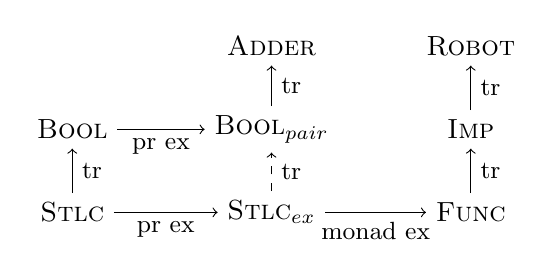
\begin{tikzpicture}[x=6pt,y=3pt,yscale=1,xscale=1]
%uncomment if require: \path (0,300); %set diagram left start at 0, and has height of 300

\node (STLC) at (-2,10) {\textsc{Stlc} };
\node (Bool) at (-2,20) {\textsc{Bool} };
\node (Boolp) at (10,20) {\textsc{Bool}$_\text{pair}$};
\node (Adder) at (10,30) {\textsc{Adder} };
\node (STLCex) at (10,10) {\textsc{Stlc}$_\text{ex}$};
\node (Ref) at (22,10) {\textsc{Func} };
\node (Imp) at (22,20) {\textsc{Imp} };
\node (Robot) at (22,30) {\textsc{Robot} };

\draw[->] (STLC) -> node[right] {\small tr} (Bool); 
\draw[->] (Bool) -> node[below] {\small pr ex} (Boolp);
\draw[->] (STLC) -> node[below] {\small pr ex} (STLCex);
% \draw[->] (STLC) -- node[below] {\small pr ex} (STLC-|STLCex) 
%  -> node[right] {\small tr} (STLCex);
\draw[->] (STLCex) -> node[below] {\small monad ex} (Ref); 
%\draw[->] (Ref) -> node[below] {\small monad ex (IO)} (RefIo);
\draw[->] (Ref) -> node[right] {\small tr} (Imp); 
\draw[->] (Imp) -> node[right] {\small tr} (Robot); 
\draw[->] (Boolp) -> node[right] {\small tr} (Adder); 
\draw[->, dashed] (STLCex) -> node[right] {\small tr} (Boolp); 
\end{tikzpicture}

  \caption{Languages for Examples}
  \label{fig:langs}
\end{figure}

%  implementing some languages based on \STLC. 
We start with meta-extensions on \STLC.
Language constructs pairs, sums, fixpoints and lists,
 introduced in Chapter 11 of Types and Programming Languages\cite{tapl} are tested.
And let bindings and ascription are implemented by translation rules.
We name the new language as \STLCex.
% In this language, we will talk about the impact of fixpoints on abstraction.

Then, we introduce reference by monad extension, getting \textsc{Ref}.
Taking \textsc{Ref} as the host language,
 we implement an imperative language \textsc{Imp}.
% The point we should care about in \textsc{Imp} is that,
%  recursive translation rules are declared in $\<while>$.
% As an extension of our framework,
%  we will discuss weak-abstraction semantic derivation.

After that, we make \textsc{Ref} support I/O, getting \RefIO.
Based on \RefIO, we implement a DSL named \textsc{Robot}.
The language assumes that a robot is located at some starting coordinates,
 and users can control its movement, or print out its position with commands.
In this example, We will talk about how to access ``global variables'' in the translation rules.

\subsection{\STLCex: Fixpoint}

Fixpoint is a common approach to implement recursion in functional programming language.
As a primitive language construct, the evaluation rule and typing rule of $\<fix>$ are specified:
\begin{align*}
  \EE{\<fix>~e} & \cqq \Let{λx:t.e_1}{\EE{e}} \EE{e_1[\<fix>~(λx:t.e_1)/x]} \\
  \TT{\<fix>~e} & \cqq \TT{e}:(t_1->t_2\mid t_1=t_2 |> t_1). 
\end{align*}

Since an expression with substituion are evaluated,
 the evaluation rule is not structural.
And as mentioned above, nonstructural evaluation rule should be considered how to maintain abstraction.
\todo{}

\subsection{\textsc{Imp}: Recursive Translation Rules}

Our \textsc{Imp} language is defined by translation rules based on \textsc{Ref},
 which means the use of variables should be reference-based.
Therefore, the syntax of \textsc{Imp} here is slightly different from the general language.
First, the declarations and initial values of variables are necessary.
For example, a legal \textsc{Imp} program is
\[ \<let>~x=\<ref>~1~\<in>~x:=!x+1; !x \]
And $x:=1;x:=x+1;x$ is not permitted for $x$ not in scope.
Also, we find that what is assigned in the declaration must be a reference to some expression.
In order to simulate the syntax of declaration in common imperative language,
 we can define syntactic sugar $\<var>$ shown in Fig. \ref{fig:imp}.
The semicolon is used as part of the syntax of the declaration, to ensure that $x$ is valid in $e_2$.

Second, in \textsc{Imp}, the left-hand side of an assignment must be a variable
 and the any variable at right-hand side refers to the value stored in it (a location).
Regretfully, we are not able to simplify this by translation rules,
 and explicit dereferences are essential.
A solution is to distinguish such $x$ by the parser, and transform to $!x$ in abstract syntax tree automatically.
We still write dereferences in the following discussion.

\begin{figure}
  \begin{align*}
    \<var>~x=e_1; e_2 & => \<let>~x=\<ref>~e_1~\<in>~e_2 \\
    \<when>~e_1~e_2 & => \<if>~e_1~e_2~() \\
    e_1 +\!\! = e_2 & => e_1 := !e_1 + e_2 \\
    \<while>~e_1~\<do>~e_2~\<end> & => \<if>~e_1~(e_2; \<while>~e_1~\<do>~e_2~\<end>)~()
  \end{align*}
  \caption{Translation Rules for \textsc{Imp}}
  \label{fig:imp}
\end{figure}

Some other common language constructs in \textsc{Imp} are defined in Fig. \ref{fig:imp}.
But $\<while>$, whose definition does not satisfy requirement \ref{req:no-recursion}, is our concern.
The semantic derivation algorithm will fail:
\begin{align*}
  & \EE{\<while>~e_1~\<do>~e_2~\<end>} \\ 
  \cqq~~ & \dhl{\EE{\<if>~e_1~(e_2; \<while>~e_1~\<do>~e_2~\<end>)~()}} \\
  =~~ & \EE{e_1}:\branch{
        \<true> |> \Let{()}{\EE{e_2}} \dhl{\EE{\<while>~e_1~\<do>~e_2~\<end>}} \\&
        \<false> |> ()
    }
\end{align*}
Consider that we discard this step of expansion, the evaluation rule of $\<while>$ can be derived as follows, 
 which is not structural but correct:
\[ 
  \EE{\<while>~e_1~\<do>~e_2~\<end>} \cqq \EE{e_1}:\branch{
    \<true> |> \Let{()}{\EE{e_2}} \EE{\<while>~e_1~\<do>~e_2~\<end>} \\&
    \<false> |> ()
  } 
\]
Because $\<while>$ itself is a language construct in the DSL,
 we can think of it as satisfying weak abstraction if we keep it in the evaluation rule.
The more serious problem is the type derivation.
It is reasonable that $\<while>$ has a recursive evaluation,
 but the typing of $\<while>$ should not be.
If the above approach is applied, an error typing rule is generated:
\begin{align*}
  \TT{\<while>~e_1~\<do>~e_2~\<end>} \cqq~
  & \Let{\<bool>}{\TT{e_1}} \Let{\<unit>}{\TT{e_2}} \\
  & \Let{t_2}{\TT{\<while>~e_1~\<do>~e_2~\<end>}} \<unit>:(t_3 \mid t_2=t_3 |> t_2)
\end{align*}
In this instance, the typing rule must be specified manually.

% More problem arise when \textsc{Imp} is used as a host language.
% When a language construct is translated to $\<while>$,
%  abstraction is difficult to guarantee.
% For example, $\<for>$ can be defined as:
% \[ \<for>~(e_1;e_2;e_3)~\<do>~e_4 => e_1;\<while>~e_2~\<do>~(e_4;e_3)~\<end> \]


\subsection{\textsc{Robot}: Limitation on Global Variables}

The goal of this language is to achieve simple control of robots in a two-dimensional plane.
A sample program of \text{Robot} is:
\[ \mathit{robot~5~5~\{ up, up, right, whereAmI, left, whereAmI \}} \]
where $\mathit{robot}~5~5\{...\}$ declares a robot with a starting point of $(5,5)$,
and the braces contain a series of commands to be executed on the robot, splitted by comma.
Some commands are used to control the movement of the robot,
 and command $\mathit{whereAmI}$ will print current position.

As a natural idea, we record the current position of the robot via the global variables $x$ and $y$.
Then each command reads and manipulates global variables,
 and comma is defined as sequencing.
These language constructs are defined as follows:
\begin{align*}
  \<robot>~e_1~e_2~\{e\} & => \<let>~x=\<ref>~e_1,y=\<ref>~e_2~\<in>~e \\
  e_1,e_2 & => e_1;e_2 \\
  \<left> & => x:=\ !x-1 \\
  \<whereAmI> & => \<print>~!x; \<print>~!y
\end{align*}
where $x$ and $y$ are literal identifiers.
But requirement \ref{req:close} is not satisfied.
Since variables without local bindings cannot be used directly in translation rules,
 it is necessary to pass the value of the variable as an argument to the language constructs or as an argument to a lambda abstraction.
Hence, $\<left>$ can be expressed as
\[ \<left> => λpos:(\<Rf>~\<int>)\times (\<Rf>~\<int>). ~(\<fst>~pos)~ \texttt{-=}~ 1; pos \]
Note that $\<left>$ returns $pos$ to keep passing on the ``global'' state.
Then, the comma operator is actually the composition of the functions.
Some selected translation rules for \textsc{Robot} are given in Fig. \ref{fig:robot}.

\begin{figure}
  \begin{align*}
    \<robot>~e_1~e_2~\{e\} & => e~(\<ref>~e_1,\<ref>~e_2) \\
    e_1,e_2 & => λpos:(\<Rf>~\<int>)\times (\<Rf>~\<int>). ~e_2~(e_1~pos) \\
    \<left> & => λpos:(\<Rf>~\<int>)\times (\<Rf>~\<int>). ~(\<fst>~pos)~ \texttt{-=}~ 1; pos \\
    % \<right> & => λpos:(\<Rf>~\<int>)\times (\<Rf>~\<int>). ~(\<fst>~pos)~ \texttt{+=}~ 1; pos \\
    % \<down> & => λpos:(\<Rf>~\<int>)\times (\<Rf>~\<int>). ~(\<snd>~pos)~ \texttt{-=}~ 1; pos \\
    % \<up> & => λpos:(\<Rf>~\<int>)\times (\<Rf>~\<int>). ~(\<snd>~pos)~ \texttt{+=}~ 1; pos \\
    \<whereAmI> & => λpos:(\<Rf>~\<int>)\times (\<Rf>~\<int>). \<print>~!(\<snd>~pos); \<print>~!(\<fst>~pos); pos
  \end{align*}
  \caption{Translation Rules for \textsc{Robot}}
  \label{fig:robot}
\end{figure}


\section{Related Work}

Our work on language lifting for DSL is related to the work on abstraction maintenance, meta-language design, and DSL implementation.

\paragraph{Abstraction Maintenance.}
We are primarily related to Resugar's work \cite{resugar}.
Resugaring is the lifting of evaluation sequence of expressions contains syntactic sugar.
The syntactic sugar here is similar to our translation rules.
A language containing syntactic sugar, called surface language;
 and the original language, called core language.
They are respectively correspond to our DSL and the host language.
An expression in a surface language is translated into the core language and evaluated in the core language first.
Then, for each expression in the host evaluation sequence,
 check whether it can be resugared to surface language using the reverse rules.
The expressions resugared are shown to users as the evaluation sequence of the surface language.
Their algorithm holds stronger properties than ours: \textit{emulation} and \textit{coverage}.
Emulation is an enhancement of correctness,
 which requires each expression in surface language evaluation sequence can be desugared into an expression in the host language evaluation sequence.
Coverage is a requirement that the evaluation process be as explicitly complete as possible to the user.
Since our current work has not yet touched on small step evaluation, it is not possible to discuss the properties associated with the evaluation sequence.
We consider providing the evaluation sequences as future work.
On the other hand, we are maintaining abstraction by making the language standalone and is done statically before program execution.
The Resugaring approach can be seen as a filtering of useful information dynamically, which is less efficient when it contains complex syntactic sugars, or when a program contains a large number of syntactic sugars.
In terms of error message reporting, we can specify which language construct caused the evaluation error, whereas resugaring can only provide error messages for the host language.
Other related work for evaluation, the main related work is how to correspond the transformed program back to the source in optimization and debugging \cite{abs-1,abs-2,abs-3}.

Other work about resugaring is also very relevant to us \cite{infer-scope,lazy-desg}.
Another main related work is typing rules inference \cite{infer-types}.
Similar to our approach, the typing rules of the host language are treated as white boxes, and the typing rules of the DSL are statically derived.
After these rules have been derived, the host language can actually be removed.
Our approach to deriving rules can be naturally generalized to types and has been implemented.
For practicality, the method of inferring typing rules support a wider range of syntactic sugars.
For example, pattern-based syntactic sugar, such as list-comprehension is allowed,
 while we only allow for unique translation rules to be defined for each DSL construct.
Also, this work introduces mechanisms such as \texttt{calc-type} to avoid users explicitly writing derivable types in the surface language (e.g., types in let binding)
And related work on typing \cite{type-sound,type-sound-1}, guarantees the soundness of type system for syntactic sugar.

\paragraph{Meta-language Design.}
Our meta-language is designed built upon the skeletal semantics \cite{skeleton},
 which can capture the behaviour of a language construct in a single rule.
By providing different interpretation,
 the skeletal semantics can build consistency between abstract and concrete interpretations.
K-framework \cite{K-framework}, Ott \cite{Ott} also allow users to define the semantics formally.
The semantics defined in K is rewrite-based, using matching logic.
For ease to use, K provides an executable interpreter and a program verifier.
Ott provides a meta-language to write semantics concisely and compiles these definition to Coq code.
The focus of these tools is on the formalization and verification of the language itself.
And our meta-language design concentrates on the feasibility of language lifting.

\paragraph{DSL Implementation.}
There is a long history of DSL implementation \cite{MartinDSL,when-how-dsl}.
Our translation rules are similar to macros and syntactic sugar.
Distinguish from selecting the appropriate host language based on the DSL design,
 we put more emphasis on the gradual expansion of the host language to append required features \cite{MoggiMeta}.
The expression problem \cite{expr-problem} is orthogonal to our problem.
The goal of expression problem is the extensibility both in data structure and interpretations,
 keeping the existing modules intact.
Instead, we directly expand the existing data structure definition for translation rules,
 which is not allowed in the expression problem.
Our approach is on top of the host language and is neither deep or shallow embedding.

\section{Conclusion}

In this paper, we propose a framework to lift language for domain-specific languages.
The key idea of the method is to derive semantics for DSL to maintain abstraction,
 in order to ensure DSL standalone.
Following this idea, we define a meta-language to describe the evaluation and type rules.
We select a pure functional programming language \STLC{} as the host language.
And base on \STLC, users can extend the host language to support new vocabularies and language features
 and specify the DSL constructs by translation rules.
We restrict the rules for the host language and the translation rules separately.
And the correctness and abstraction of the semantic derivation algorithm is proved.
In addition, we implement the tool Osazone,
 which is shown to be useful to develop DSLs.

 

\bibliographystyle{ACM-Reference-Format}
\bibliography{ref.bib}

\appendix
\section{Proofs}

\subsection{Proof of Lemma \ref{lemma:sig-bone}}

\begin{lemmaapp}
  Support $\cb$ is a closed bone. Then:
  \[ \cb \rr{X} v \quad\miff\quad \dd(\cb) \rr{X} v. \]
\end{lemmaapp}

\begin{proof}
  By induction on a derivation of $\cb \rr{X} v$. 
  The \textsc{Expression} and \textsc{Filter} cases are immediate, since $\dd(\cb)=\cb$.
  The other cases are shown as follows:

  Case \textsc{Hook}: let $\cb=\EE{e}$, where $e$ is a closed expression.
  We consider each case separately according to $e$:
  \begin{itemize}
    \item $e$ is a base expression: $\dd(b)=b$;
    \item $e=c~\cexp_1\cdots \cexp_n$: we have $\EE{e} \rr{X} v$, iff $L[e] \rr{X} v$.
      Furthermore, according to the definition of $\dd$, 
      we can find an environment $Σ$ and a rule $\EE{\mexp}\cqq b_1$ in $L$, such that $Σ(\mexp) = e$, $\dd(\EE{e})=\dd(Σ(b_1))$.
      According to the definition, $Σ(b_1)=L[e]$.
      Then $\dd(\EE{e})=\dd(L[e])$.
      Since $e$ is a closed variable, $Σ(b_1)$ is a closed bone.
      By the induction hypothesis, $L[e]\rr{X} v$ iff $\dd(L[e])\rr{X} v$.
      Then, $\EE{e}\rr{X} v$, iff $\dd(\EE{e})\rr{X} v$.
  \end{itemize}

  Case \textsc{LetIn}: let $b=\Let{pat}{b_1} b_2$.
    Then $b\rr{X} v$, iff the following judgements are satisfied:  
    \[ b_1\rr{X_1}v_1 \quad Σ=match(pat,v_1) \quad Σ(b_2)\rr{X_2}v_2 \quad X=X_1;X_2, \]
     where $Σ(b_2)$ is a closed bone.
    By the induction hypothesis and Lemma \ref{lemma:del-sig}, we have
    \begin{align*}
      b_1\rr{X_1}v_1    & \quad\miff\quad \dd(b_1)\rr{X_1} v_1, \\
      Σ(b_2)\rr{X_2}v_2 & \quad\miff\quad Σ(\dd(b_2))\rr{X_2}v_2
    \end{align*} 
    Therefore, we can apply rule \textsc{LetIn} to conclude
    \[ \Let{pat}{\dd(b_1)} \dd(b_2) \rr{X} v \]
    whose left-hand side equals to $\dd(b)$.

  Case \textsc{Branch}: Similar.
\end{proof}


\end{document}
\endinput
